\chapter{The HiSPARC Experiment}

\section{Detector}

% Using scintillators with PMTs provide good particle detection efficiency, \SI{100}{\percent} of energetic leptons are detected, also some gammas are seen.
The detector consists of two main components which perform the detection. The scintillator, which emits light when charged particles pass through it, and the Photomultiplier tube (\pmt) which converts the scintillation photons into an electric signal.

\subsection{Detector components}

% Scintillator size and material
Scintillators have been selected as detection material. This is a relatively cheap material with high reliability and excellent efficiency. The scintillator is a sheet of \SI[product-units=power]{100 x 50 x 2}{\centi\meter} made from BC-408 \cite{sgc2011bc408}. The BC-408 material has good timing properties and light output for charged particles.

% PMT size and type
The chosen photomultiplier tube \cite{et2010pmt} is a compact \SI{29}{\milli\meter} (\SI{25}{\milli\meter} effectively) diameter and \SI{~11}{\centi\meter} long (depends on the power supply) \pmt. The quantum efficiency of the biakali photocathode is \SI{25}{\percent} for the wavelength of maximum emission of the scintillator, which is \SI{425}{\nano\meter}. The \pmts contain a number of high gain caesiated antimony (SbCs) dynodes. The \pmts are very efficient at amplifying faint light pulses to measurable electric signals. Several brands and types of \pmts have been used. At first \pmts (including power supply) were sourced from Electron Tubes, ET Enterprises and Sens-Tech, later new \pmts were constructed using Hamamatsu tubes with a \nikhef power supply. The \nikhef power supply is also compatible with the previously used tubes, and can serve to replace a failed power supply.

Besides these the detector construction consists of several other components. An isosceles triangle with a squared top made from polymethylmethacrylate (PMMA) as light guide. The light guide has the following measurements a base of \SI{50}{\centi\meter}, legs of \SI{71.5}{\centi\meter}, and the thickness is \SI{2.2}{\centi\meter} (the top is also \SI{2.2}{\centi\meter} wide). The light guide is glued to the scintillator using Optical Cement \cite{sgc2014bc600}. A little adapter piece from square to round shape (same material as light guide) is attached to the square top of the triangle with Optical Cement and the round window of the \pmt with optical tape [ref type?]. This construction is wrapped in thin, \SI{30}{\micro\meter}, aluminium foil with patches of thicker aluminium foil at the corners of the scintillator, to prevent the sharp edges from piercing the thin foil. This is then wrapped in \SI{0.5}{\milli\meter} thick light-tight black pond foil to keep light out and protect the aluminium foil from outside influences.

% Material is mostly 'off the shelf'. Construction/assembly can be performed by students.
All components are readily available, off the shelf, from suppliers and not specifically designed for \hisparc.

\begin{figure}
    \centering
    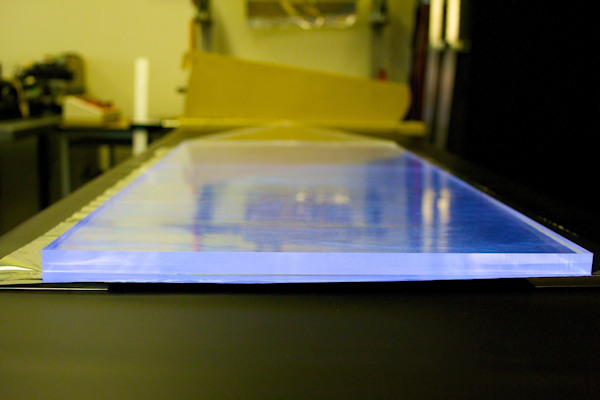
\includegraphics[width=0.6\textwidth]
                    {plots/station/ADL_115651.jpg}
    \caption{Show a schematic/photo of detector, indicating the various components.}
    \label{fig:schematic_detector}
\end{figure}

% Detector is protected by skibox from weather and is secured in place by weights.
The final detector dimensions (approximately) \SI[product-units=power]{200 x 50 x 3}{\centi\meter} fit well in the chosen detector casing, namely, roof boxes (in Dutch generally referred to as `ski box'). These can be securely fastened and are designed to withstand all kinds of weather. Access to the detector for maintenance is also easy. Also with maintenance in mind, the optical tape with which the \pmt is attached allows it to be easily replaced. In \cref{fig:detector_in_skibox} a detector in a skibox is shown.

\begin{figure}
    \centering
    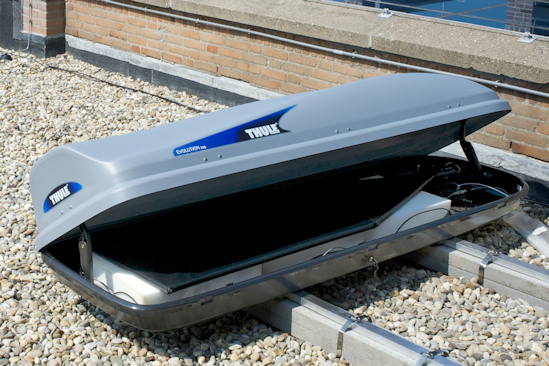
\includegraphics[width=0.6\textwidth]
                    {plots/station/ADL_105036.jpg}
    \caption{Detector in a skibox on the roof.}
    \label{fig:detector_in_skibox}
\end{figure}

\subsection{The scintillator}

% How Scintillator works
Charge particles loose energy in the scintillator in interactions with the base of the scintillator, polyvinyltoluene. Ionisation is the main source of energy loss for energetic charged particles (electrons, muons). The base will emit photons which are rapidly absorbed by the fluor of the scintillator, anthracene. The fluor then emits light at a lower wavelength, to which the scintillator is more transparent. Some of this light will reach the \pmt.

% Most shower muons/electrons are minimum ionising particles (mips) and have similar energy loss in the detectors, given by Bethe-Bloch (spread on energy loss given by Landau).
The average energy deposited by the particle going through the detector is described by the Bethe-Bloch formula. This gives the amount of energy lost by the particles per \si{\gram\centi\meter\squared} of the material it passes through. However, the interactions in which the particles loose energy is a statistical process, the energy loss is not a fixed number but a distribution, the Landau distribution. The ionisation energy loss (predicted by Bethe-Bloch) for both electrons and muons reaches a minimum value at some point. Muons and electrons at this energy (\SI{325e6}{\eV} and \SI{e6}{\eV} respectively) are referred to as \textit{minimum ionising particles} (\mip). In \cref{fig:bethe-bloch} the energy loss for electrons and muons is shown as a function of their energy. Shown are the total losses (grey), losses due to ionisation (black), and other loss processes. The ionisation losses are the only ones of real interest, since those result in the detectable scintillation light.

\begin{figure}
    \centering
    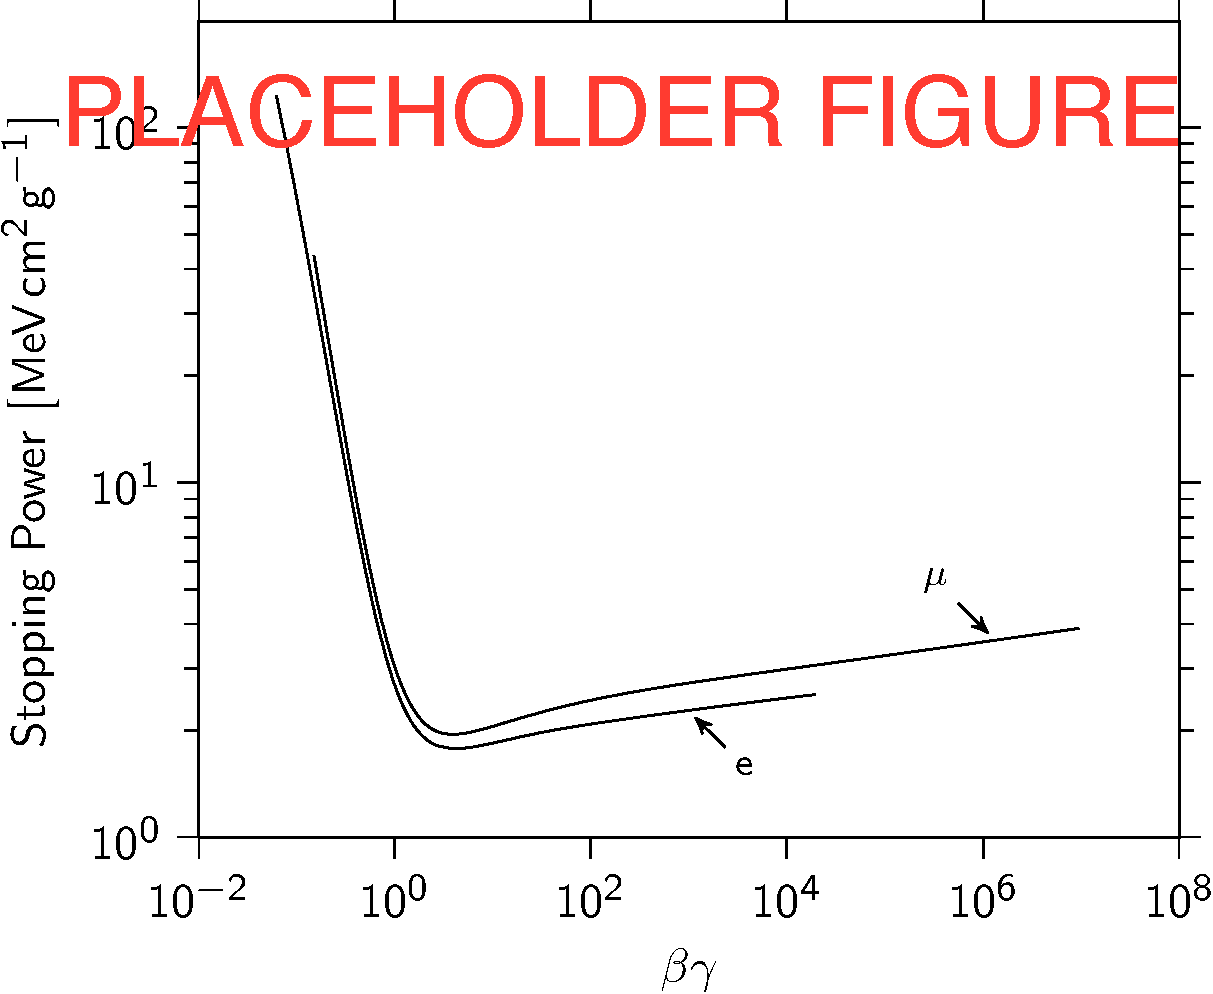
\includegraphics[width=0.6\textwidth]
                    {plots/station/bethe-bloch}
    \caption{Expected ionization energy loss in the scintillator for electrons and muons as a function of their energy. Calculated with the Bethe-Bloch formula (use eV[/c] horizontal scale (two scales?) or keep beta gamma.}
    \label{fig:bethe-bloch}
\end{figure}

The scintillator is \SI{2}{\centi\meter} thick, however, many particles have a longer path through it because they travel at an angle. This increases the expected mean energy loss. The path can also be shorter if the particle passes through one of the sides of the scintillator, but due to the large area of the detector relative to its thickness the chance of that happening is low.

% Signal transport efficiency not uniform for the detector due to geometry.
The light emitted along the path of the particle is transmitted in random directions. Depending on the angle at which the emitted photons hit the outer edges of the scintillator there is a chance that they will be reflected back or leave the scintillator. The entire detector is wrapped in aluminium foil to attempt to reflect those photons back into the scintillator. To detect the photons they need to hit the photocathode of the \pmt. To get to the \pmt they need to pass from the scintillator through a layer of optical glue, the light guide, another layer of optical glue, a small piece of light guide, and a layer of optical tape to reach the \pmt. During this most photons will be reflected a number of times. For \SI{1}{\mip} approximately 30000 photons [check.] are emitted, the fraction that reach the \pmt depend on the location in the scintillator where the particles are emitted. A 2D Monte Carlo simulation of the detector predicts the transmission efficiency from locations in the scintillator to the \pmt \cite{steijger2010mc}. The resulting transmission efficiency distribution is shown in\cref{fig:signal_response}. Also the travel time of the photons to the \pmt varies depending on the location of emission and the emission direction. In \cref{fig:transport_time} the distribution of transport times is shown, the time is the arrival time of the 15th photon producing a photoelectron at the \pmt. This is taken instead of the first because the signal threshold used for detection is greater than the signal of one photoelectron. The effects of these distributions on the reconstruction accuracy are discussed later.

\begin{figure}
    \centering
    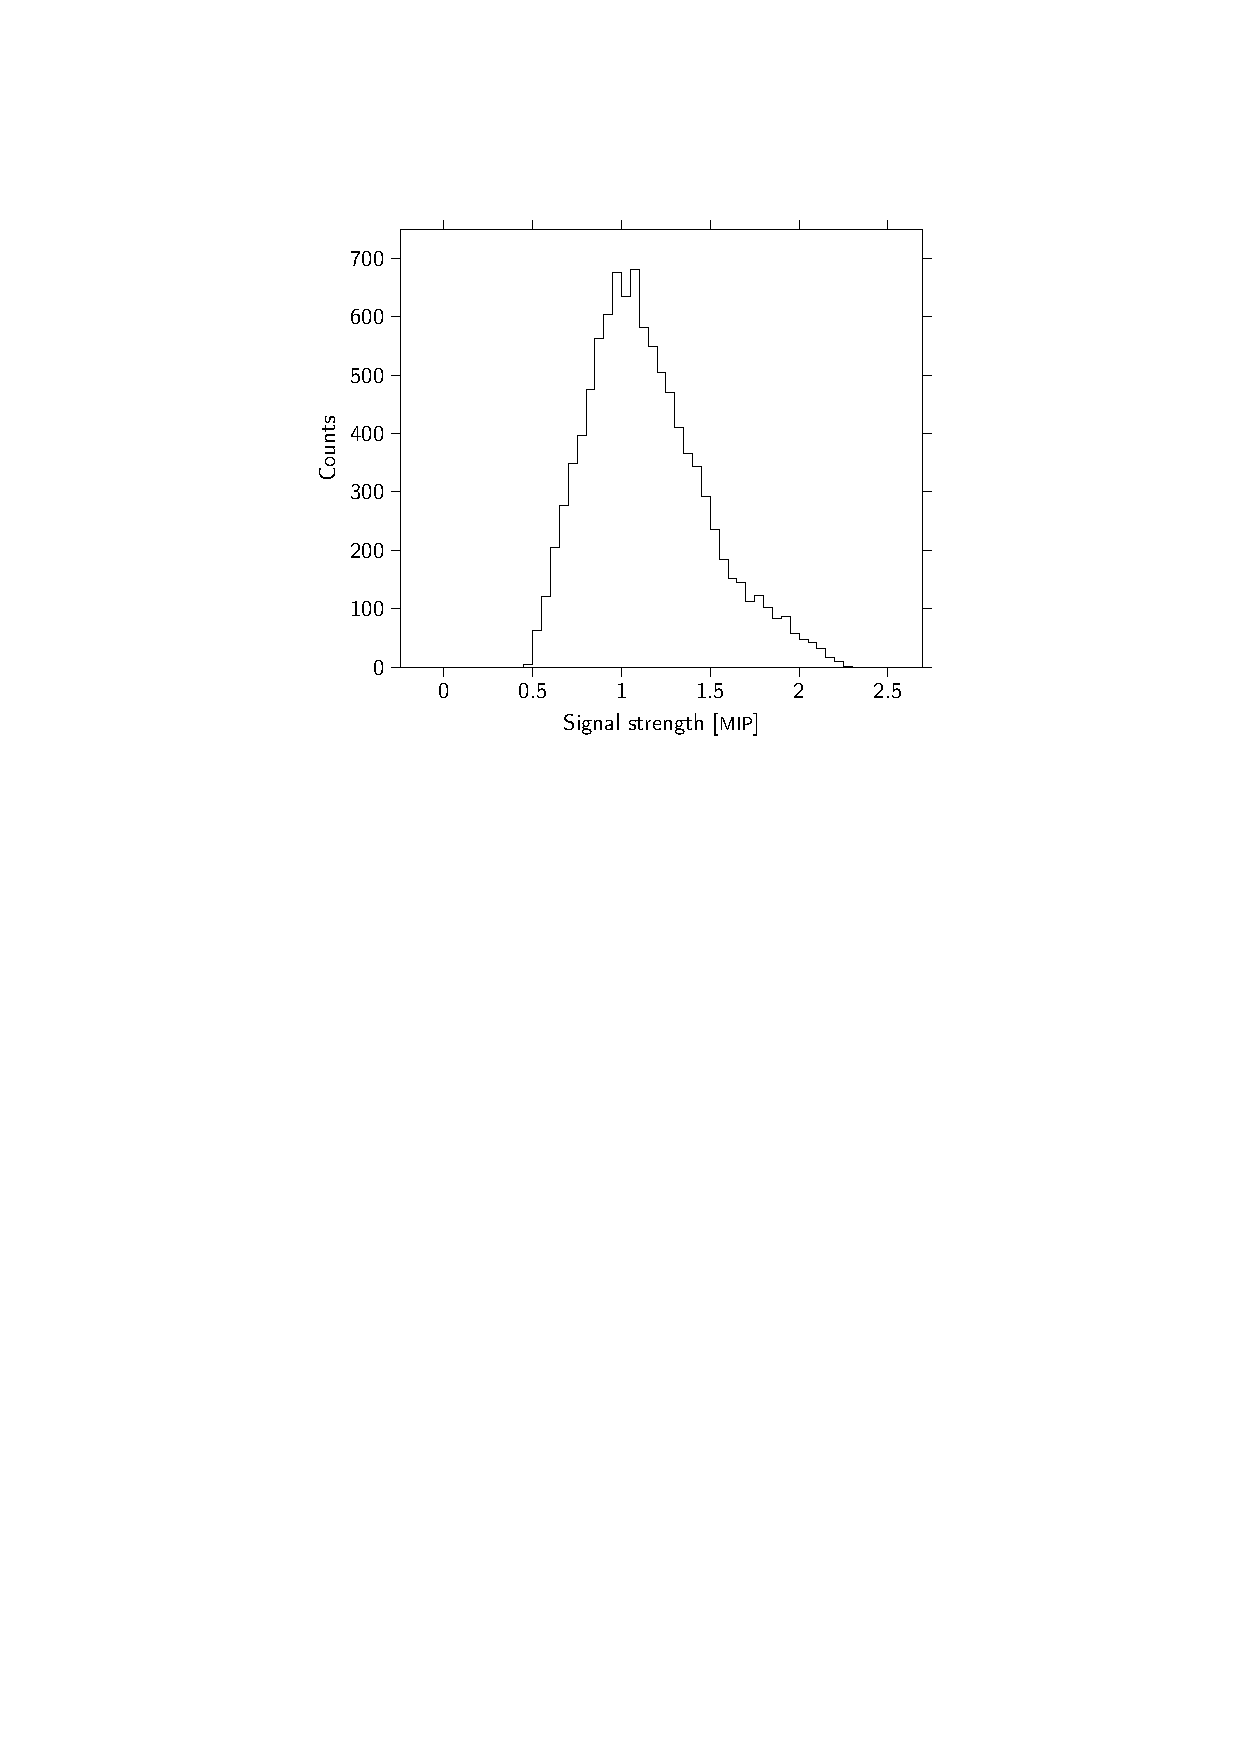
\includegraphics[width=0.6\textwidth]
                    {plots/station/signal_response}
    \caption{Signal response distribution for the detector. The detector response is statistically modelled. The effect of particle angle of incidence can be accounted for by dividing the x-axis by $cos \theta$.}
    \label{fig:signal_response}
\end{figure}

\begin{figure}
    \centering
    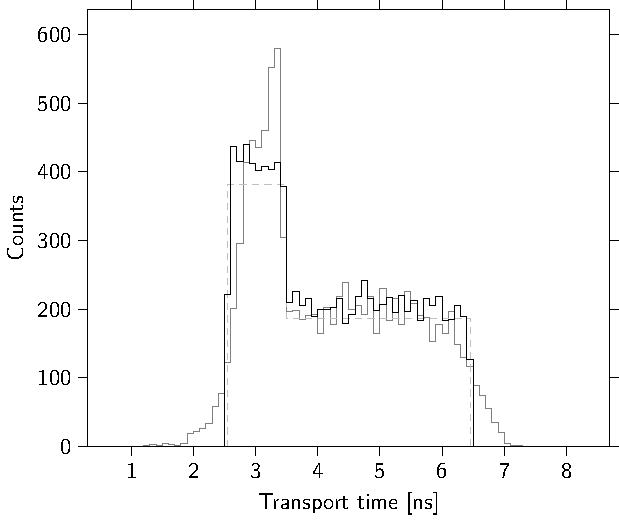
\includegraphics[width=0.6\textwidth]
                    {plots/station/transport_time}
    \caption{Transport time distribution for the detector. The scintillation light has to reach the PMT from the point of impact, the travel time depends on the impact location, this is the distribution for the entire detector.}
    \label{fig:transport_time}
\end{figure}


\subsubsection{Gammas in the scintillator}

Energetic photons can also deposit energy in the scintillator due to Compton scattering and pair creation. However, the cross sections for these interactions is very low. A \SI{e6}{\eV} photon  has a mean free path greater than \SI{10}{\centi\meter}, which increases further for higher energy photons, see fig [By Jos/Tom]. Despite the low detection chance, the large number of photons in an air shower makes them statistically relevant.

For photons the interactions by which it produces detectable signals are .., and pair production. In case electrons are produced, those will proceed in the usual way.


\subsection{\pmt}

% How PMT works
The photomultiplier tube has a front window with a photocathode. When this is hit by a photon an electron can be knocked free, due to the photoelectric effect. The electron is then pulled along electric field lines which direct it to a dynode. The electron will cause multiple electrons to be emitted from the dynode, these electrons are then pulled to the next dynode, which has a higher positive potential. Each electron impacting the second dynode will cause the release of more electrons, which are accelerated towards the next dynode, and so on. At the end the electrons fall on the anode which is connected to the readout. This is shown in \cref{fig:pmt_schematic}.

\begin{figure}
    \centering
    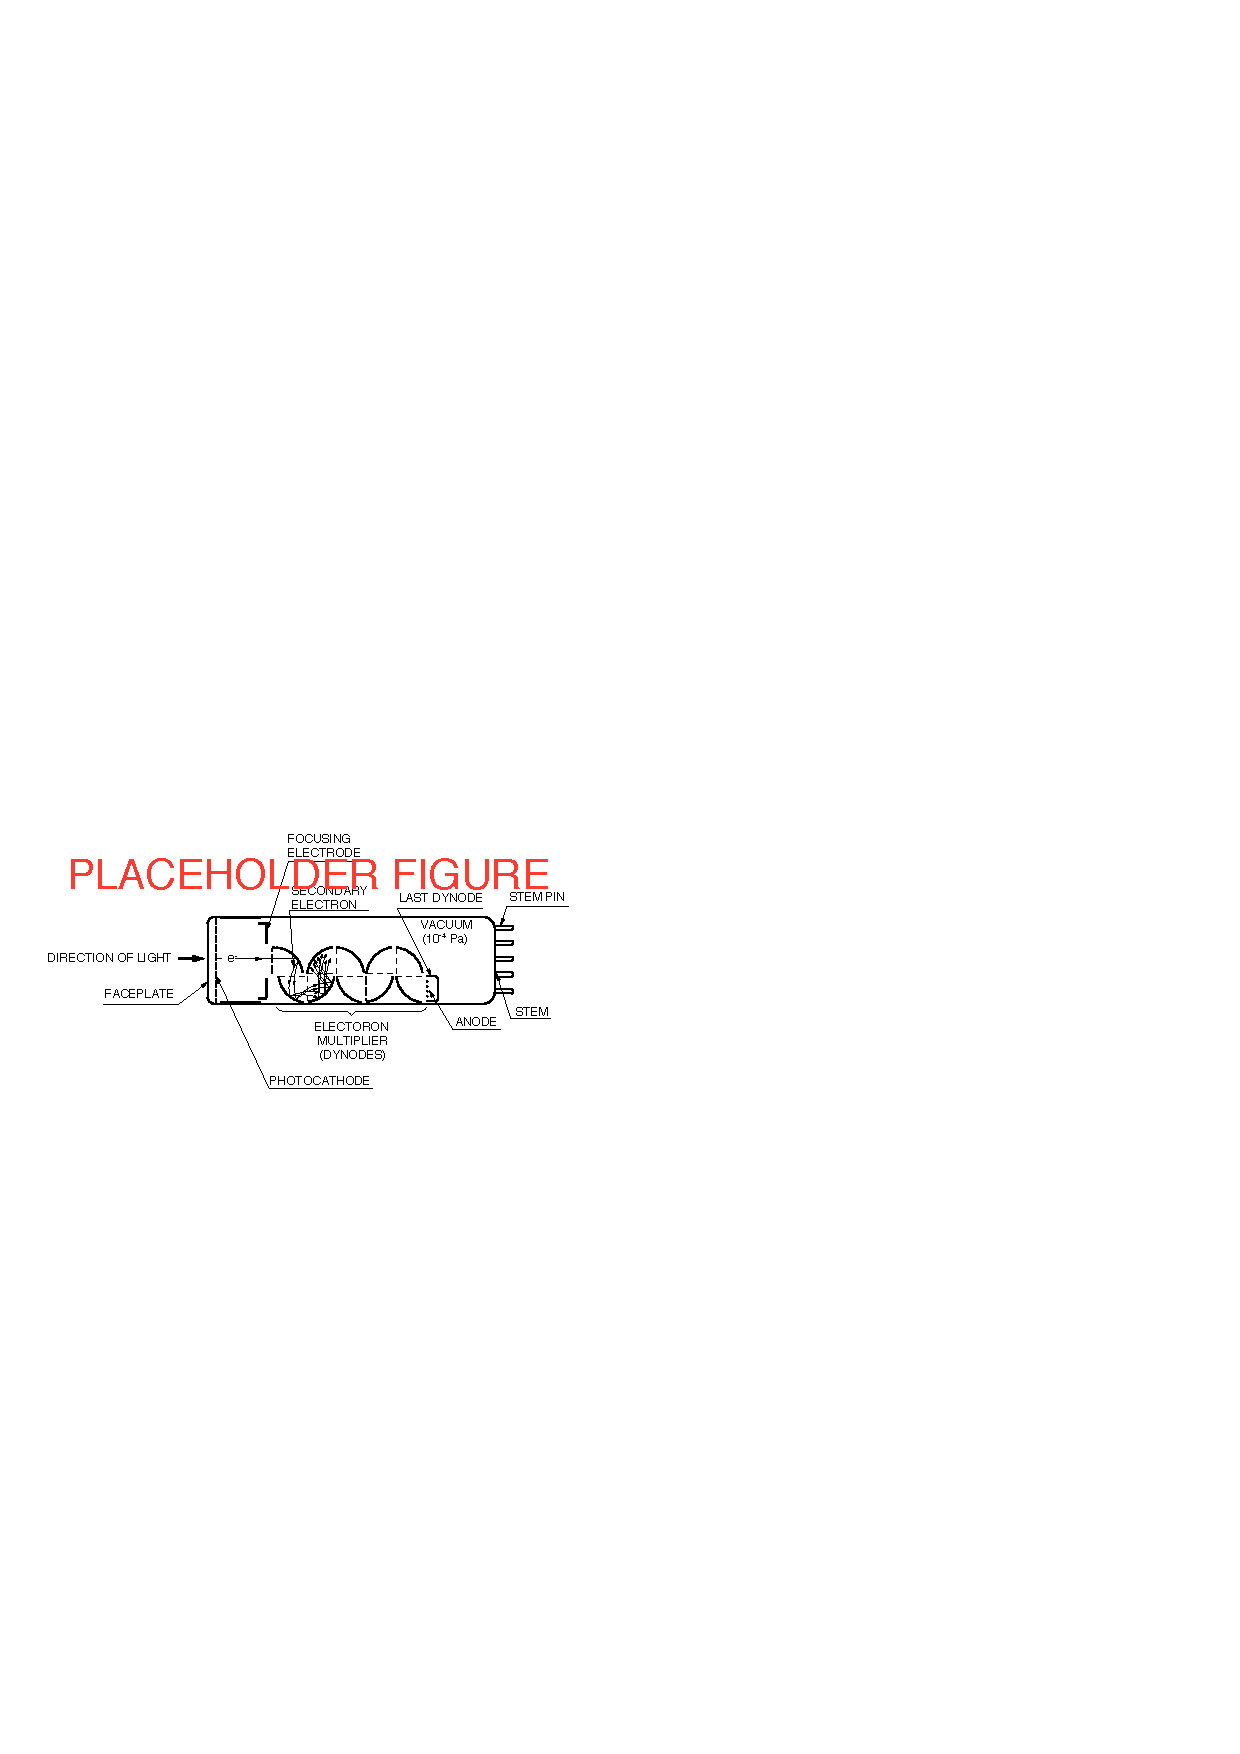
\includegraphics[width=0.6\textwidth]
                    {plots/station/pmt_schematic}
    \caption{Schematic crosssection of a \pmt.}
    \label{fig:pmt_schematic}
\end{figure}

% PMT gain, fluctuations in gain..
The \pmts which are used have 11? (ET/SensTech) and 12? (Hamamatsu) dynodes, this number affects the gain of the \pmt. If each electron causes \num{3} electrons to be released from a dynode then every electron falling on the first dynode will result in $3^{n_{\mathrm{dynodes}}} = \mathcal{O}(10^6)$ electrons at the anode. The number of electrons emitted by a dynode for each electron that falls on it is not a fixed number. This results in a variation in the output signal for each single photoelectron. This can easily vary a factor of 2, if for instance the first dynode emits either 2 or 4 electrons instead of 3. It is more likely to happen at a later dynode because more interaction occur at those. Typical variations are of the order of \SI{10}{\percent}. By changing the voltage on the dynodes the gain of the \pmt can be tuned, with a higher voltage resulting in a higher gain. The relation between gain and voltage is not linear [perhaps a fig, or at least a ref].

% Signal strength is used for particle density, need to be able to distinguish between different number.
Both the scintillator and \pmt can handle multiple particles simultaneously and will produce correspondingly higher signal output. The integrated signal strength should be the sum of two individual particles. Given the signal distribution for single particles given by the Landau distribution combined with the transport efficiency one particle will in some (how often?) produce a signal equal or larger than the most probable signal strength of two particles. In \cref{fig:ph_histogram_contrib} an example of the expected pulse height histogram is shown including the contributions from gammas, and multiple leptons. The widths of the contributions are due to the particle inclination, Landau distribution, transmission efficiency, and \pmt variation. The first peak gives the most probable value (MPV) for the pulse height of a single lepton. An approximation of the number of particles can be made by comparing a measured value to the MPV. The position of the MPV is dependent on the efficiency of the detector, by changing the voltage on the \pmt the position of the MPV can be tuned. Ideally the MPV is approximately \SI{150}{\mV}. If it is lower it is difficult to distinguish the lepton contribution from the gamma spectrum and the MPV will be hard to determine. If the MPV is at a much higher value the \pmt ages more quickly and the dynamic range [in number of particles..] will be reduced.

\begin{figure}
    \centering
    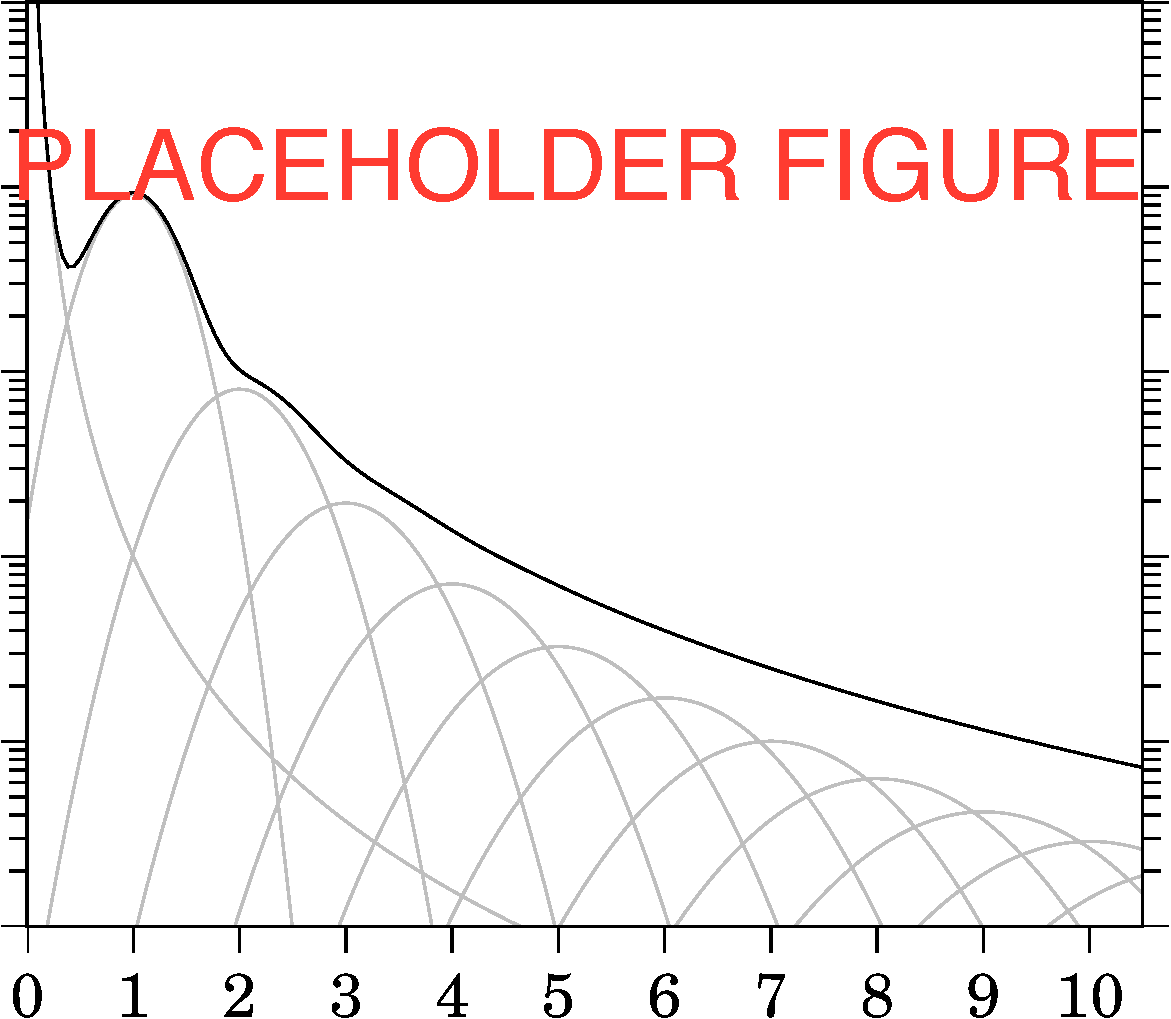
\includegraphics[width=0.6\textwidth]
                    {plots/station/ph_histogram_contrib}
    \caption{Overlap between pulse integral contributions from multiple mips in one event, the with of each contribution is due to Landau distribution and transport efficiency.}
    \label{fig:ph_histogram_contrib}
\end{figure}

% Fast ADC readout of the PMT provides accurate timing.
Each \pmt is readout with \adcs at a sample rate of \SI{2.5}{\ns}. An example of a readout is shown in \cref{fig:trace}. With this high sample rate the signal shape of individual particles is unraveled. Subsequent signals from particles later in the shower front can be distinguished, and the shower rise time can be examined. With \SI{2.5}{\ns} the timing resolution is close to timing the uncertainty caused by the shower front rise time and the detector transport time. An even higher sample rate would not achieve much better timing resolution.

\begin{figure}
    \centering
    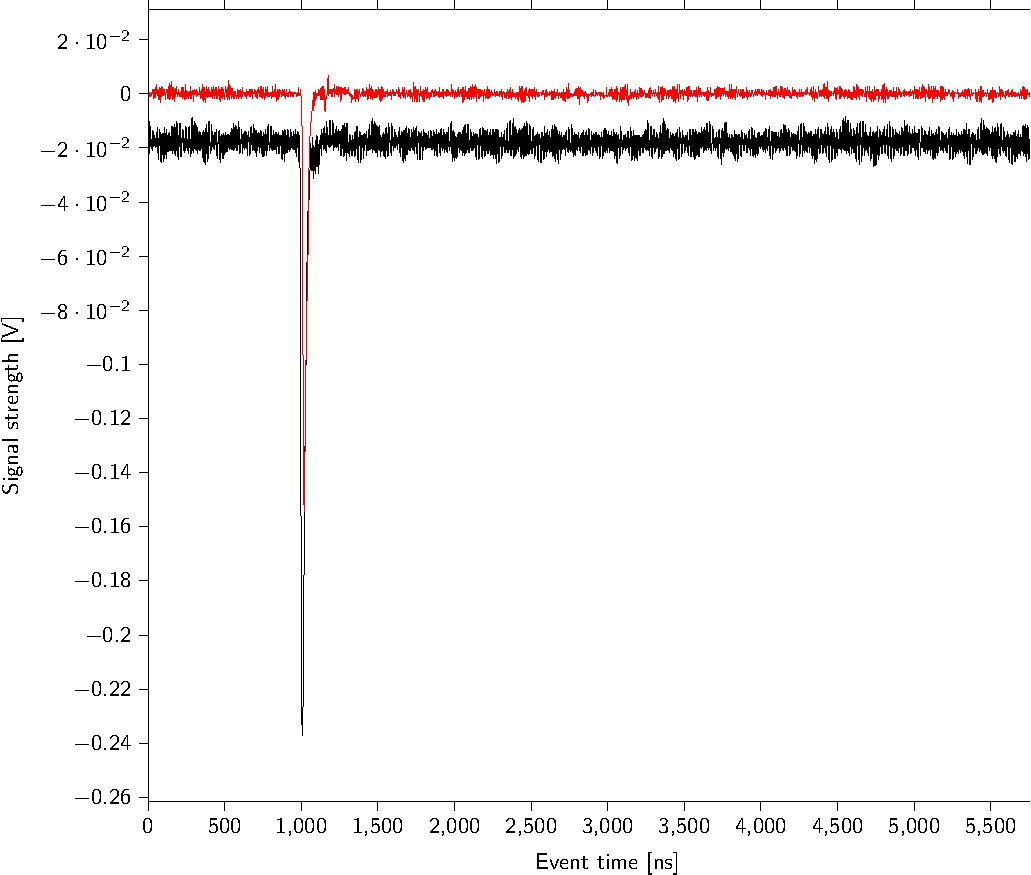
\includegraphics[width=0.6\textwidth]
                    {plots/station/trace}
    \caption{An example trace readout of the \pmt. The signal has the height of one \mip, so most likely one lepton was detected.}
    \label{fig:trace}
\end{figure}







\section{Signal performance of a detector}
\label{sec:detector-signal}

\subsection{Scintillator uniformity}

Monte Carlo simulation of signal transport in the detector predicts a non-uniform signal transmission for particles passing through different positions of the detector. This is experimentally confirmed by coincidence tests using a \SI[product-units = repeat]{1 x 1}{\centi\meter} scintillator connected to a \pmt and the standard detector. The small detector was then placed on various location on top of the large detector. Particles passing through both detectors are selected using a coincidence trigger. This way the position of the particle in the large detector is known and the efficiency at specific points can be determined. In \cref{fig:scintilator_transmission_compared} the results from the experiment and the simulation for the various positions are compared.

\begin{figure}
    \centering
    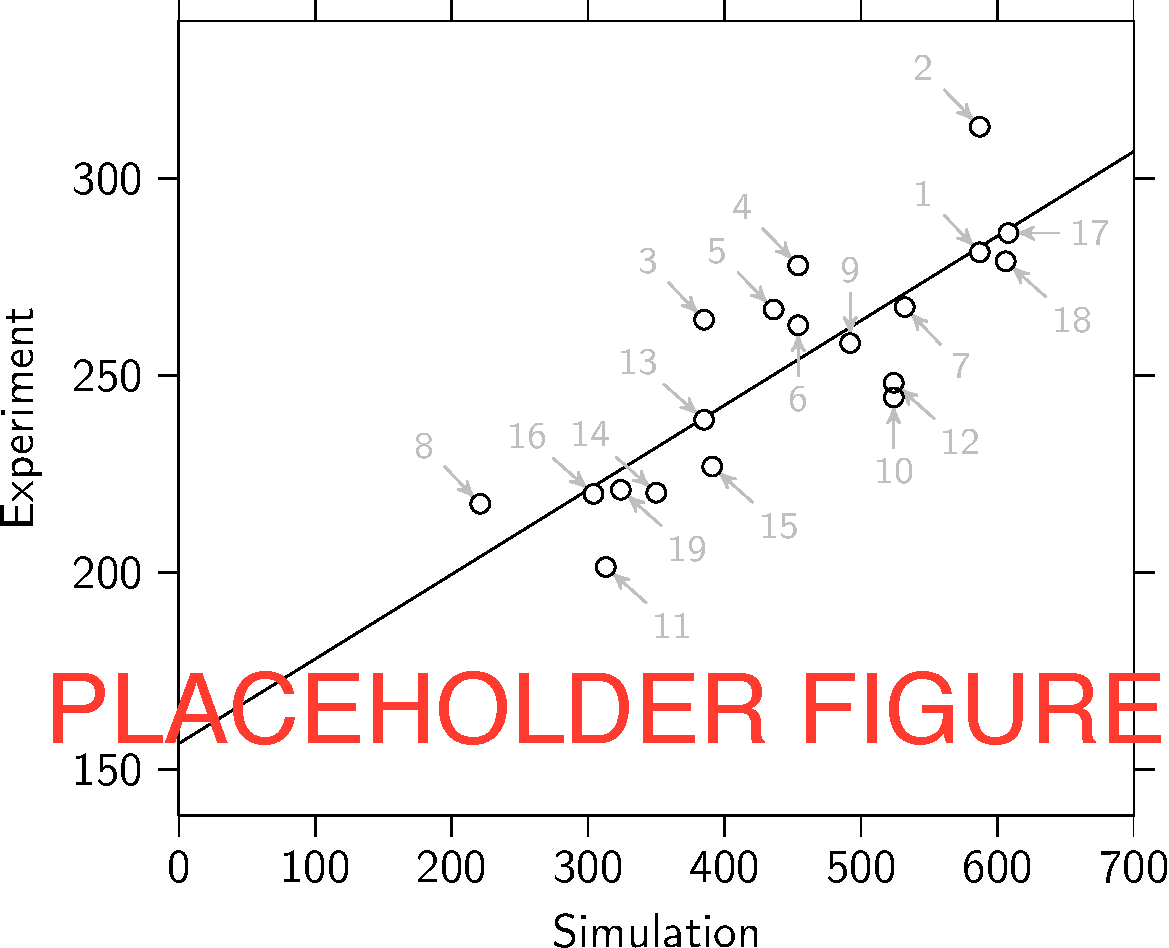
\includegraphics{plots/station/scintilator_transmission_compared}
    \caption{Correlation between the transmission efficiency for different positions in the scintillator between a real HiSPARC detector and the simulated one. The difference can be explained by the aluminium foil in which the detector is wrapped is not taken into account in the simulation. Moreover, some of the positions are in locations where the simulation predicts a significant gradient.}
    \label{fig:scintilator_transmission_compared}
\end{figure}

In the detector simulation the distribution in \cref{fig:signal_efficiency} is used to simulate the signal strength caused by each particle in a detector. First combining the Bethe-Bloch formula and energy-straggling results in the Landau distribution, for vertical particles. The Landau distribution gives the amount of energy lost by particles which pass through the detector. In the simulations the exact location in the detector is ignored. Therefore, the Landau distribution is convolved with the transmission efficiency distribution of the detectors. The resulting distribution can be scaled by $\cos{\theta}^{-1}$ for particles arriving at angles in the detector.

\begin{figure}
    \centering
    % \usepackage{tikz}
% \usetikzlibrary{arrows}
% \usepackage{pgfplots}
% \pgfplotsset{compat=1.3}
% \usepackage[detect-family]{siunitx}
% \usepackage[eulergreek]{sansmath}
% \sisetup{text-sf=\sansmath}
% \usepackage{relsize}
%
\tikzsetnextfilename{externalized-signal_efficiency}
\pgfkeysifdefined{/artist/width}
    {\pgfkeysgetvalue{/artist/width}{\defaultwidth}}
    {\def\defaultwidth{ .67\linewidth }}
%
%
\begin{sansmath}
\begin{tikzpicture}[
        font=\sffamily,
        every pin/.style={inner sep=2pt, font={\sffamily\smaller}},
        every label/.style={inner sep=2pt, font={\sffamily\smaller}},
        every pin edge/.style={<-, >=stealth', shorten <=2pt},
        pin distance=2.5ex,
    ]
    \begin{axis}[
            axis background/.style={  },
            xmode=normal,
            ymode=normal,
            width=\defaultwidth,
            axis equal=false,
            %
            title={  },
            %
            xlabel={ Signal strength [\si{\mip}] },
            ylabel={ Counts },
            %
            xmin={  },
            xmax={  },
            ymin={ 0.0 },
            ymax={  },
            %
            xtick={  },
            ytick={  },
            %
            tick align=outside,
            max space between ticks=40,
            every tick/.style={},
            axis on top,
        ]

        






    
    % Draw series plot
    \addplot[no markers,solid,const plot] coordinates {
        (0.0, 0)
        (0.05, 0)
        (0.1, 0)
        (0.15, 0)
        (0.2, 0)
        (0.25, 0)
        (0.3, 0)
        (0.35, 0)
        (0.4, 0)
        (0.45, 5)
        (0.5, 62)
        (0.55, 121)
        (0.6, 205)
        (0.65, 277)
        (0.7, 349)
        (0.75, 397)
        (0.8, 476)
        (0.85, 563)
        (0.9, 604)
        (0.95, 676)
        (1.0, 635)
        (1.05, 681)
        (1.1, 582)
        (1.15, 549)
        (1.2, 505)
        (1.25, 471)
        (1.3, 411)
        (1.35, 365)
        (1.4, 344)
        (1.45, 292)
        (1.5, 235)
        (1.55, 184)
        (1.6, 152)
        (1.65, 145)
        (1.7, 112)
        (1.75, 122)
        (1.8, 103)
        (1.85, 83)
        (1.9, 86)
        (1.95, 58)
        (2.0, 47)
        (2.05, 43)
        (2.1, 32)
        (2.15, 17)
        (2.2, 10)
        (2.25, 1)
        (2.3, 0)
        (2.35, 0)
        (2.4, 0)
        (2.45, 0)
    };







    \end{axis}
\end{tikzpicture}
\end{sansmath}

    \caption{Signal distribution for one particle. This distribution gives the signal from a single particles passing straight through a random location of the scintillator. The distribution scales with $\cos{\theta}^{-1}$.}
    \label{fig:signal_efficiency}
\end{figure}


\subsection{\pmt linearity}

In an EAS many more than one particle may pass through a detector. The response of the \pmt to different signal sizes needs to be investigated to determine the accuracy with which the number of particles can be reconstructed. Ideally the output of the \pmt grows linearly with the number of photons impacting its photocathode. Large signals from the \pmt, capable of saturating the \adc, are expected to occur dozens of times a day. However, in the data we find that some \pmts never produce signals that saturate the \adc. Calibration tests have been performed on several \pmts to test their output given a known input signal.


\subsection{PMT calibration}
\label{sub:pmt_calibration}

A setup has been created to test the linearity of \pmts using LED light flashes. A bundle of 24 optical fibers, each connected to a LED, are fed into a cap which directs the light at the window of a \pmt. The LEDs can be triggered simultaneously to produce a short (\SI{20}{\ns}) pulse. This is similar to a pulse generator, but with light. The intensity of light produced on the \pmt by a single fiber is comparable to one or two \mip in a detector. The pulse-to-pulse intensity typically fluctuates by \SI{50}{\percent}. Taking the average over hundreds of pulses gives a very stable result.

\begin{figure}
    \centering
    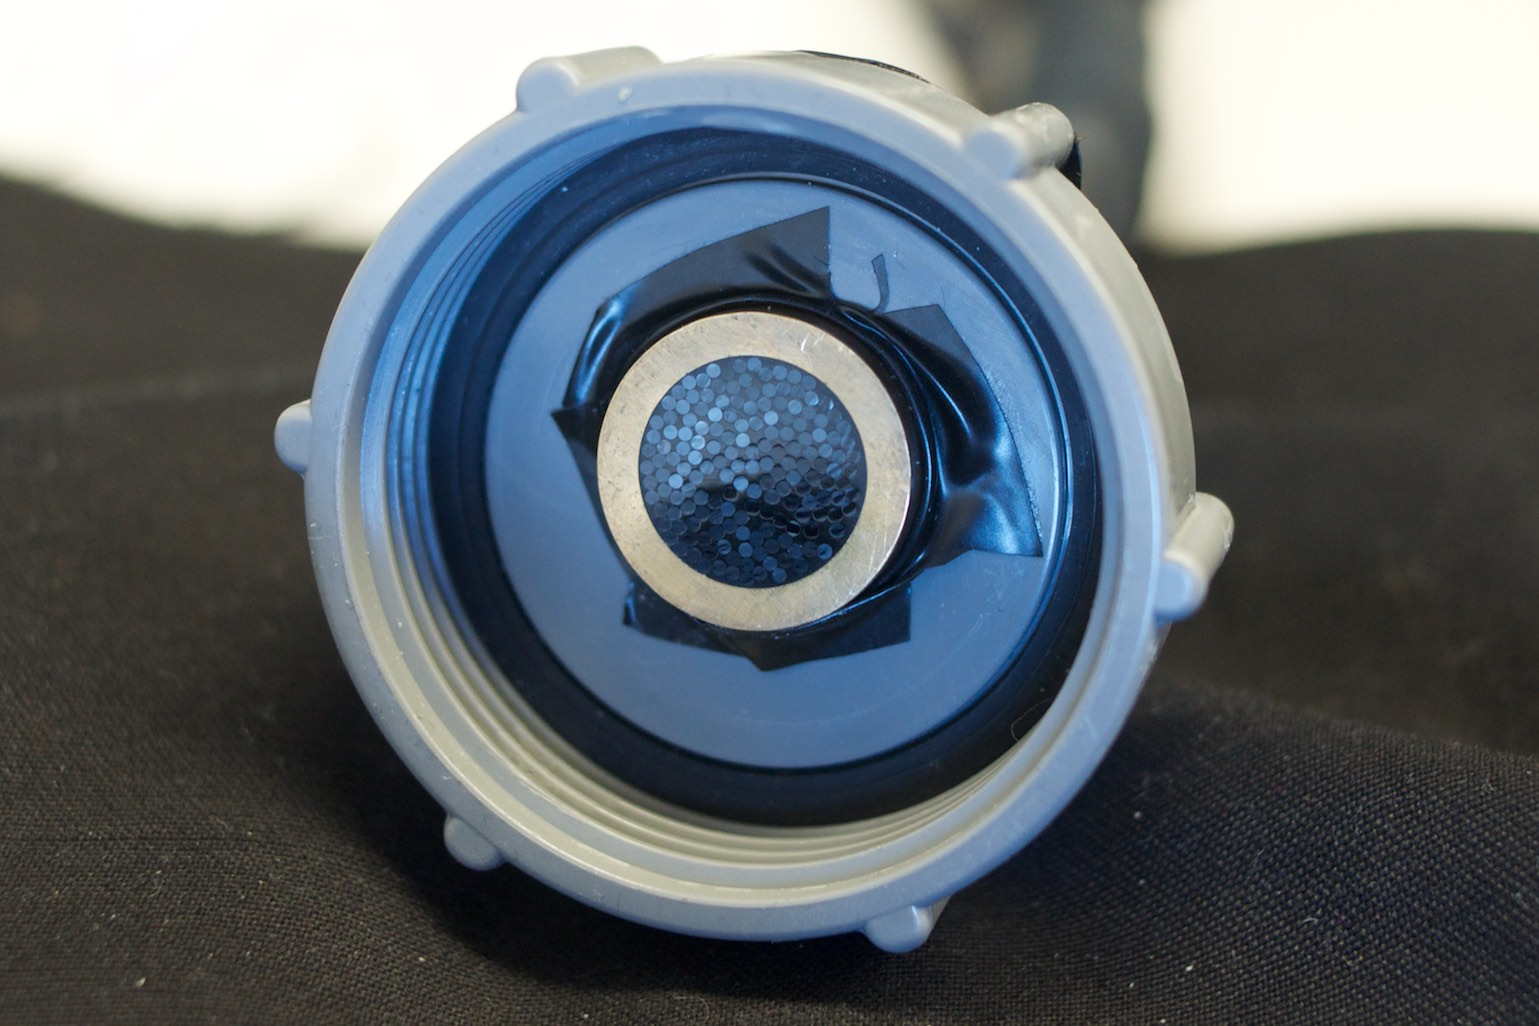
\includegraphics[width=.45\linewidth]{plots/station/ARN_085351.jpg}
    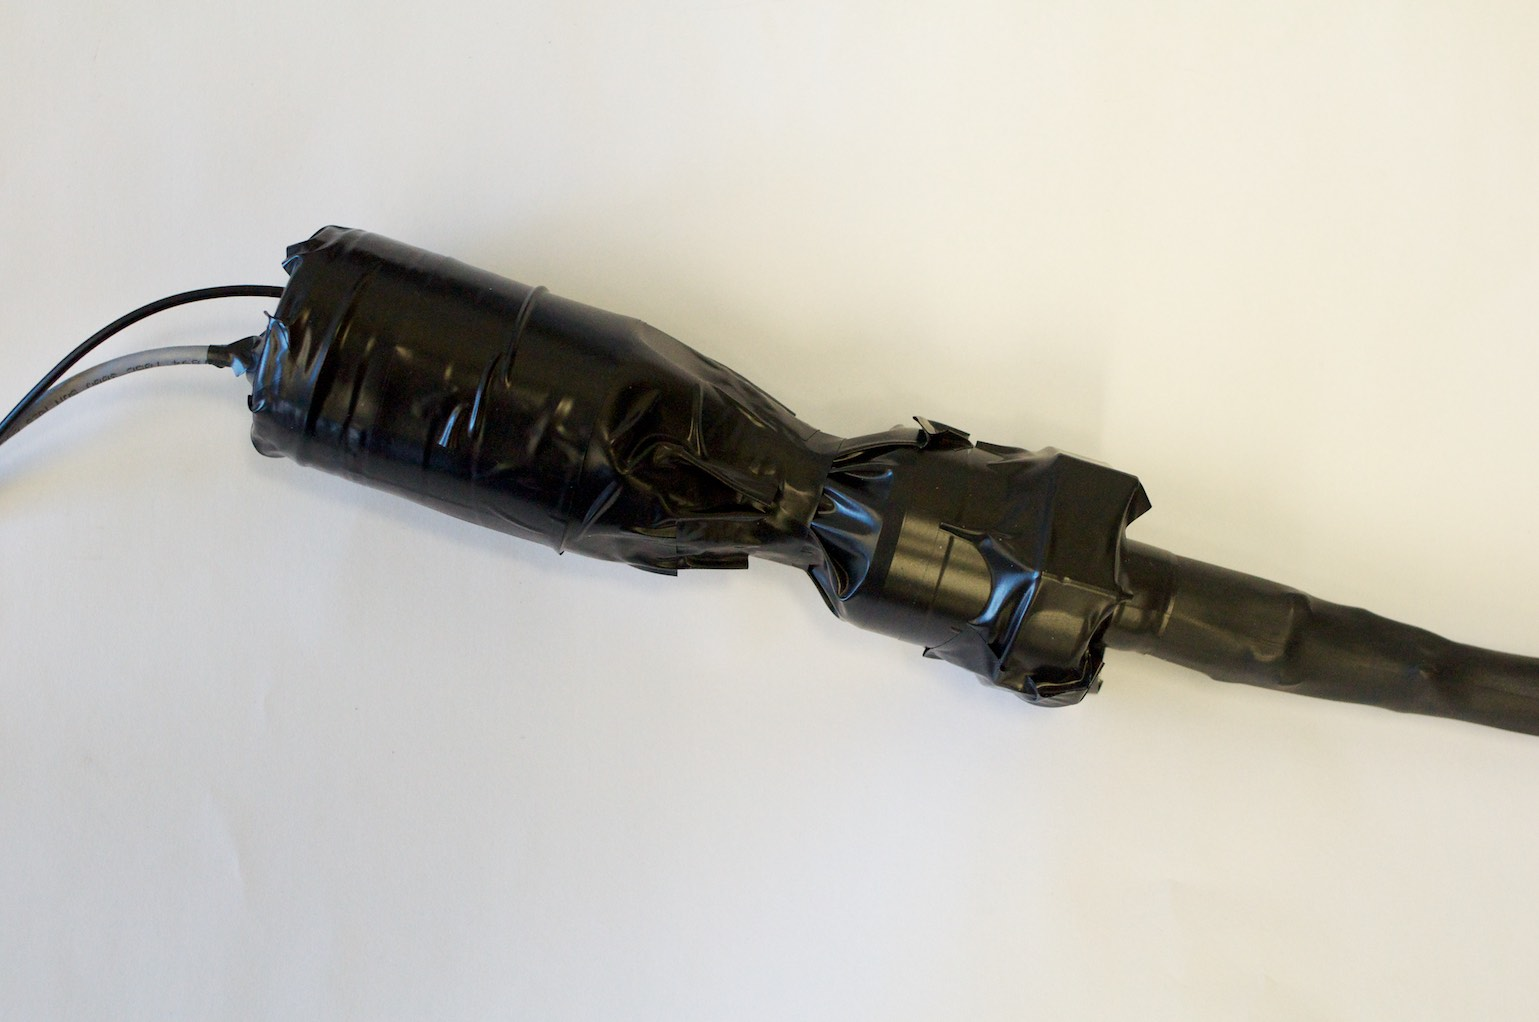
\includegraphics[width=.45\linewidth]{plots/station/ARN_085349.jpg}
    \caption{Here the setup for the PMT tests is shown. The first photo shows the fibers in the bundle. The second photo shows the bundle connected to the \pmt, wrapped light tight with tape.}
    \label{fig:pmt_test_setup}
\end{figure}

The mean intensity of the individual fibers is not equal. For each \pmt the mean intensity of each individual fiber is determined. This is done by disconnecting and darkening the other fibers. This makes it possible to determine the input signal when multiple fibers are connected. This is expected to be the sum of the individual signals. Possible time delays between the pulses might make the resulting pulses wider instead of higher, so not only the pulse height is examined but also the pulse integral. Any subset of the 24 fibers can be used simultaneously. Signals with and expected \pmt output pulse over \SI{5}{\volt} are possible with the full bundle of fibers, with the \pmt is still at normal operating voltage.

An oscilloscope is used to readout the \pmt signal. This allows for easy averaging of multiple signals and to readout signals larger than \SI{2}{\volt}. The oscilloscope measures the signal's pulse height and integral.

In \cref{fig:linearity_pmts} the results of two \pmt tests are shown. The \senstech \pmt already start to be non-linear before the pulse height reaches \SI{1}{\volt}. With increased signal input it just barely reaches \SI{2}{\volt}. The \nikhef \pmt on the other hand is linear over the entire range that was measured. The tests confirm that the \nikhef produced \pmt power supplies can supply enough current to saturate the \hisparc electronics. Larger input signals were not possible with the used setup, so it remains unclear at what point it will be unable to keep up. The non-linear curve can be fitted by the following equation, as described in \cite{icecube2010pmt}.

\begin{equation}
    \ln V_{\mathrm{in}} = \ln V +
                          \frac{p_0 \left(\frac{V}{p_1}\right)^{p_2}}
                               {\left(1 - \frac{V}{p_1}\right)^{\frac{1}{4}}}
\end{equation}

Where $V$ is the measured output signal and $V_{in}$ the input. The parameters ($p_{1,2,3}$) have no physical meaning.

\begin{figure}
    \centering
    % \usepackage{tikz}
% \usetikzlibrary{arrows,external}
% \usepackage{pgfplots}
% \pgfplotsset{compat=1.3}
% \usepackage[detect-family]{siunitx}
% \usepackage[eulergreek]{sansmath}
% \sisetup{text-sf=\sansmath}
% \usepackage{relsize}
%
    \tikzsetnextfilename{externalized-linearity_compared}
\pgfkeysifdefined{/artist/width}
    {\pgfkeysgetvalue{/artist/width}{\defaultwidth}}
    {\def\defaultwidth{ .6\linewidth }}
%
    \pgfkeysifdefined{/artist/height}
        {\pgfkeysgetvalue{/artist/height}{\defaultheight}}
        {\def\defaultheight{ .6\linewidth }}
%
\begin{sansmath}
\begin{tikzpicture}[
        font=\sffamily,
        every pin/.style={inner sep=2pt, font={\sffamily\smaller}},
        every label/.style={inner sep=2pt, font={\sffamily\smaller}},
        every pin edge/.style={<-, >=stealth', shorten <=2pt},
        pin distance=2.5ex,
    ]
    \begin{axis}[
            axis background/.style={  },
            xmode=normal,
            ymode=normal,
            width=\defaultwidth,
                height=\defaultheight,
            scale only axis,
            axis equal=true,
            %
            title={  },
            %
            xlabel={ Sum individual LED pulse heights [V] },
            ylabel={ Multiple-LED pulse height [V] },
            %
            xmin={ 0 },
            xmax={ 6005 },
            ymin={ 0 },
            ymax={ 6005 },
            %
            xtick={ 0, 1000, 2000, 3000, 4000, 5000, 6000 },
            ytick={ 0, 1000, 2000, 3000, 4000, 5000, 6000 },
            xticklabels={  0, 1, 2, 3, 4, 5, 6 },
            yticklabels={  0, 1, 2, 3, 4, 5, 6 },
            xticklabel style={  },
            yticklabel style={  },
            %
            tick align=outside,
            max space between ticks=40,
            every tick/.style={},
            axis on top,
            point meta min={  },
            point meta max={  },
                colormap={coolwarm}{
                    rgb255(0cm)=( 59, 76,192);
                    rgb255(1cm)=( 98,130,234);
                    rgb255(2cm)=(141,176,254);
                    rgb255(3cm)=(184,208,249);
                    rgb255(4cm)=(221,221,221);
                    rgb255(5cm)=(245,196,173);
                    rgb255(6cm)=(244,154,123);
                    rgb255(7cm)=(222, 96, 77);
                    rgb255(8cm)=(180,  4, 38)},
        ]





    % Draw series plot
    \addplot[mark=*,mark options=white,only marks] coordinates {
            (5050, 5050)
            (4671, 4723)
            (4379, 4396)
            (3953, 3950)
            (3466, 3560)
            (3030, 3150)
            (2600, 2686)
            (2075, 2140)
            (1685, 1746)
            (1194, 1224)
            (722, 716)
            (348, 318)
    };


    % Draw series plot
    \addplot[mark=*,only marks] coordinates {
            (412, 325)
            (572, 550)
            (754, 730)
            (934, 860)
            (1130, 1000)
            (1289, 1120)
            (1529, 1267)
            (1719, 1339)
            (1959, 1453)
            (2203, 1545)
            (2405, 1605)
            (2655, 1712)
            (2875, 1776)
            (3077, 1844)
            (3240, 1877)
            (3539, 1960)
            (3721, 1983)
            (3951, 2036)
            (4406, 2097)
            (4782, 2150)
            (4932, 2170)
    };


    % Draw series plot
    \addplot[mark=o,only marks] coordinates {
            (5050, 5050)
            (4671, 4723)
            (4379, 4396)
            (3953, 3950)
            (3466, 3560)
            (3030, 3150)
            (2600, 2686)
            (2075, 2140)
            (1685, 1746)
            (1194, 1224)
            (722, 716)
            (348, 318)
    };


    % Draw series plot
    \addplot[no markers,solid] coordinates {
            (326.895910995, 325.0)
            (330.671772439, 328.69739479)
            (334.449956614, 332.394789579)
            (338.230505781, 336.092184369)
            (342.013462519, 339.789579158)
            (345.798869719, 343.486973948)
            (349.586770591, 347.184368737)
            (353.377208656, 350.881763527)
            (357.170227752, 354.579158317)
            (360.965872032, 358.276553106)
            (364.764185963, 361.973947896)
            (368.565214329, 365.671342685)
            (372.369002228, 369.368737475)
            (376.175595075, 373.066132265)
            (379.9850386, 376.763527054)
            (383.797378851, 380.460921844)
            (387.61266219, 384.158316633)
            (391.430935297, 387.855711423)
            (395.252245171, 391.553106212)
            (399.076639126, 395.250501002)
            (402.904164795, 398.947895792)
            (406.73487013, 402.645290581)
            (410.568803402, 406.342685371)
            (414.4060132, 410.04008016)
            (418.246548434, 413.73747495)
            (422.090458336, 417.434869739)
            (425.937792457, 421.132264529)
            (429.78860067, 424.829659319)
            (433.642933171, 428.527054108)
            (437.50084048, 432.224448898)
            (441.362373439, 435.921843687)
            (445.227583214, 439.619238477)
            (449.096521299, 443.316633267)
            (452.969239511, 447.014028056)
            (456.845789996, 450.711422846)
            (460.726225227, 454.408817635)
            (464.610598004, 458.106212425)
            (468.498961457, 461.803607214)
            (472.391369049, 465.501002004)
            (476.28787457, 469.198396794)
            (480.188532145, 472.895791583)
            (484.09339623, 476.593186373)
            (488.002521618, 480.290581162)
            (491.915963433, 483.987975952)
            (495.83377714, 487.685370741)
            (499.756018537, 491.382765531)
            (503.682743763, 495.080160321)
            (507.614009296, 498.77755511)
            (511.549871954, 502.4749499)
            (515.490388898, 506.172344689)
            (519.435617631, 509.869739479)
            (523.385616, 513.567134269)
            (527.340442201, 517.264529058)
            (531.300154772, 520.961923848)
            (535.264812602, 524.659318637)
            (539.23447493, 528.356713427)
            (543.209201345, 532.054108216)
            (547.189051788, 535.751503006)
            (551.174086554, 539.448897796)
            (555.164366293, 543.146292585)
            (559.159952012, 546.843687375)
            (563.160905078, 550.541082164)
            (567.167287213, 554.238476954)
            (571.179160505, 557.935871743)
            (575.196587403, 561.633266533)
            (579.219630719, 565.330661323)
            (583.248353633, 569.028056112)
            (587.282819692, 572.725450902)
            (591.323092812, 576.422845691)
            (595.36923728, 580.120240481)
            (599.421317758, 583.817635271)
            (603.479399279, 587.51503006)
            (607.543547255, 591.21242485)
            (611.613827476, 594.909819639)
            (615.69030611, 598.607214429)
            (619.773049708, 602.304609218)
            (623.862125206, 606.002004008)
            (627.957599924, 609.699398798)
            (632.059541571, 613.396793587)
            (636.168018243, 617.094188377)
            (640.283098432, 620.791583166)
            (644.404851018, 624.488977956)
            (648.533345283, 628.186372745)
            (652.6686509, 631.883767535)
            (656.810837948, 635.581162325)
            (660.959976904, 639.278557114)
            (665.116138651, 642.975951904)
            (669.279394478, 646.673346693)
            (673.449816082, 650.370741483)
            (677.62747557, 654.068136273)
            (681.812445466, 657.765531062)
            (686.004798705, 661.462925852)
            (690.204608641, 665.160320641)
            (694.41194905, 668.857715431)
            (698.626894129, 672.55511022)
            (702.849518499, 676.25250501)
            (707.07989721, 679.9498998)
            (711.318105741, 683.647294589)
            (715.564220004, 687.344689379)
            (719.818316345, 691.042084168)
            (724.080471548, 694.739478958)
            (728.350762838, 698.436873747)
            (732.62926788, 702.134268537)
            (736.916064787, 705.831663327)
            (741.211232119, 709.529058116)
            (745.514848887, 713.226452906)
            (749.826994555, 716.923847695)
            (754.147749043, 720.621242485)
            (758.477192732, 724.318637275)
            (762.815406463, 728.016032064)
            (767.162471543, 731.713426854)
            (771.518469744, 735.410821643)
            (775.883483314, 739.108216433)
            (780.257594969, 742.805611222)
            (784.640887905, 746.503006012)
            (789.033445797, 750.200400802)
            (793.435352802, 753.897795591)
            (797.846693563, 757.595190381)
            (802.267553212, 761.29258517)
            (806.698017375, 764.98997996)
            (811.138172169, 768.687374749)
            (815.588104215, 772.384769539)
            (820.047900631, 776.082164329)
            (824.517649044, 779.779559118)
            (828.997437586, 783.476953908)
            (833.487354903, 787.174348697)
            (837.987490155, 790.871743487)
            (842.497933023, 794.569138277)
            (847.018773707, 798.266533066)
            (851.550102935, 801.963927856)
            (856.092011963, 805.661322645)
            (860.644592581, 809.358717435)
            (865.207937113, 813.056112224)
            (869.782138426, 816.753507014)
            (874.367289928, 820.450901804)
            (878.963485578, 824.148296593)
            (883.570819882, 827.845691383)
            (888.189387904, 831.543086172)
            (892.819285266, 835.240480962)
            (897.460608153, 838.937875752)
            (902.113453317, 842.635270541)
            (906.777918079, 846.332665331)
            (911.454100337, 850.03006012)
            (916.142098565, 853.72745491)
            (920.842011823, 857.424849699)
            (925.553939756, 861.122244489)
            (930.277982599, 864.819639279)
            (935.014241184, 868.517034068)
            (939.762816942, 872.214428858)
            (944.523811908, 875.911823647)
            (949.297328724, 879.609218437)
            (954.083470645, 883.306613226)
            (958.882341544, 887.004008016)
            (963.694045912, 890.701402806)
            (968.518688871, 894.398797595)
            (973.356376168, 898.096192385)
            (978.207214187, 901.793587174)
            (983.071309954, 905.490981964)
            (987.948771134, 909.188376754)
            (992.839706044, 912.885771543)
            (997.744223656, 916.583166333)
            (1002.6624336, 920.280561122)
            (1007.59444616, 923.977955912)
            (1012.5403723, 927.675350701)
            (1017.50032366, 931.372745491)
            (1022.47441254, 935.070140281)
            (1027.46275195, 938.76753507)
            (1032.46545555, 942.46492986)
            (1037.48263773, 946.162324649)
            (1042.51441357, 949.859719439)
            (1047.56089883, 953.557114228)
            (1052.62221001, 957.254509018)
            (1057.6984643, 960.951903808)
            (1062.78977964, 964.649298597)
            (1067.89627465, 968.346693387)
            (1073.01806873, 972.044088176)
            (1078.15528198, 975.741482966)
            (1083.30803525, 979.438877756)
            (1088.47645015, 983.136272545)
            (1093.66064902, 986.833667335)
            (1098.86075499, 990.531062124)
            (1104.07689194, 994.228456914)
            (1109.30918449, 997.925851703)
            (1114.55775809, 1001.62324649)
            (1119.82273894, 1005.32064128)
            (1125.10425402, 1009.01803607)
            (1130.40243113, 1012.71543086)
            (1135.71739886, 1016.41282565)
            (1141.0492866, 1020.11022044)
            (1146.39822456, 1023.80761523)
            (1151.76434376, 1027.50501002)
            (1157.14777605, 1031.20240481)
            (1162.54865413, 1034.8997996)
            (1167.9671115, 1038.59719439)
            (1173.40328255, 1042.29458918)
            (1178.85730247, 1045.99198397)
            (1184.32930735, 1049.68937876)
            (1189.81943414, 1053.38677355)
            (1195.32782063, 1057.08416834)
            (1200.85460552, 1060.78156313)
            (1206.39992839, 1064.47895792)
            (1211.9639297, 1068.17635271)
            (1217.54675081, 1071.87374749)
            (1223.14853401, 1075.57114228)
            (1228.76942247, 1079.26853707)
            (1234.40956029, 1082.96593186)
            (1240.06909252, 1086.66332665)
            (1245.74816513, 1090.36072144)
            (1251.44692501, 1094.05811623)
            (1257.16552004, 1097.75551102)
            (1262.90409903, 1101.45290581)
            (1268.66281177, 1105.1503006)
            (1274.44180901, 1108.84769539)
            (1280.2412425, 1112.54509018)
            (1286.06126495, 1116.24248497)
            (1291.90203009, 1119.93987976)
            (1297.76369265, 1123.63727455)
            (1303.64640837, 1127.33466934)
            (1309.550334, 1131.03206413)
            (1315.47562734, 1134.72945892)
            (1321.42244721, 1138.42685371)
            (1327.39095348, 1142.1242485)
            (1333.38130708, 1145.82164329)
            (1339.39366999, 1149.51903808)
            (1345.42820527, 1153.21643287)
            (1351.48507707, 1156.91382766)
            (1357.5644506, 1160.61122244)
            (1363.66649219, 1164.30861723)
            (1369.79136927, 1168.00601202)
            (1375.93925039, 1171.70340681)
            (1382.11030521, 1175.4008016)
            (1388.30470453, 1179.09819639)
            (1394.52262029, 1182.79559118)
            (1400.76422561, 1186.49298597)
            (1407.02969472, 1190.19038076)
            (1413.31920307, 1193.88777555)
            (1419.63292725, 1197.58517034)
            (1425.97104507, 1201.28256513)
            (1432.33373553, 1204.97995992)
            (1438.72117883, 1208.67735471)
            (1445.13355639, 1212.3747495)
            (1451.57105089, 1216.07214429)
            (1458.03384621, 1219.76953908)
            (1464.5221275, 1223.46693387)
            (1471.03608117, 1227.16432866)
            (1477.5758949, 1230.86172345)
            (1484.14175764, 1234.55911824)
            (1490.73385965, 1238.25651303)
            (1497.35239247, 1241.95390782)
            (1503.99754898, 1245.65130261)
            (1510.66952337, 1249.34869739)
            (1517.36851116, 1253.04609218)
            (1524.09470922, 1256.74348697)
            (1530.84831578, 1260.44088176)
            (1537.62953045, 1264.13827655)
            (1544.4385542, 1267.83567134)
            (1551.27558941, 1271.53306613)
            (1558.14083984, 1275.23046092)
            (1565.03451068, 1278.92785571)
            (1571.95680856, 1282.6252505)
            (1578.90794153, 1286.32264529)
            (1585.88811909, 1290.02004008)
            (1592.89755222, 1293.71743487)
            (1599.93645335, 1297.41482966)
            (1607.00503643, 1301.11222445)
            (1614.10351688, 1304.80961924)
            (1621.23211166, 1308.50701403)
            (1628.39103923, 1312.20440882)
            (1635.58051961, 1315.90180361)
            (1642.80077437, 1319.5991984)
            (1650.05202662, 1323.29659319)
            (1657.33450107, 1326.99398798)
            (1664.64842404, 1330.69138277)
            (1671.9940234, 1334.38877756)
            (1679.3715287, 1338.08617234)
            (1686.78117108, 1341.78356713)
            (1694.22318335, 1345.48096192)
            (1701.69779996, 1349.17835671)
            (1709.20525704, 1352.8757515)
            (1716.74579244, 1356.57314629)
            (1724.31964566, 1360.27054108)
            (1731.92705796, 1363.96793587)
            (1739.56827231, 1367.66533066)
            (1747.24353344, 1371.36272545)
            (1754.95308784, 1375.06012024)
            (1762.69718377, 1378.75751503)
            (1770.47607128, 1382.45490982)
            (1778.29000224, 1386.15230461)
            (1786.13923034, 1389.8496994)
            (1794.02401111, 1393.54709419)
            (1801.94460193, 1397.24448898)
            (1809.90126205, 1400.94188377)
            (1817.89425261, 1404.63927856)
            (1825.92383665, 1408.33667335)
            (1833.99027915, 1412.03406814)
            (1842.093847, 1415.73146293)
            (1850.23480905, 1419.42885772)
            (1858.41343613, 1423.12625251)
            (1866.63000105, 1426.82364729)
            (1874.88477862, 1430.52104208)
            (1883.17804569, 1434.21843687)
            (1891.51008112, 1437.91583166)
            (1899.88116585, 1441.61322645)
            (1908.2915829, 1445.31062124)
            (1916.74161736, 1449.00801603)
            (1925.23155644, 1452.70541082)
            (1933.7616895, 1456.40280561)
            (1942.33230802, 1460.1002004)
            (1950.94370566, 1463.79759519)
            (1959.59617827, 1467.49498998)
            (1968.2900239, 1471.19238477)
            (1977.02554283, 1474.88977956)
            (1985.80303757, 1478.58717435)
            (1994.62281291, 1482.28456914)
            (2003.48517592, 1485.98196393)
            (2012.39043597, 1489.67935872)
            (2021.33890475, 1493.37675351)
            (2030.33089631, 1497.0741483)
            (2039.36672705, 1500.77154309)
            (2048.44671577, 1504.46893788)
            (2057.57118366, 1508.16633267)
            (2066.74045436, 1511.86372745)
            (2075.95485393, 1515.56112224)
            (2085.21471094, 1519.25851703)
            (2094.52035643, 1522.95591182)
            (2103.87212395, 1526.65330661)
            (2113.2703496, 1530.3507014)
            (2122.71537205, 1534.04809619)
            (2132.20753254, 1537.74549098)
            (2141.74717491, 1541.44288577)
            (2151.33464564, 1545.14028056)
            (2160.97029387, 1548.83767535)
            (2170.6544714, 1552.53507014)
            (2180.38753275, 1556.23246493)
            (2190.16983514, 1559.92985972)
            (2200.00173856, 1563.62725451)
            (2209.88360577, 1567.3246493)
            (2219.81580233, 1571.02204409)
            (2229.79869661, 1574.71943888)
            (2239.83265985, 1578.41683367)
            (2249.91806614, 1582.11422846)
            (2260.0552925, 1585.81162325)
            (2270.24471885, 1589.50901804)
            (2280.48672808, 1593.20641283)
            (2290.78170605, 1596.90380762)
            (2301.13004164, 1600.6012024)
            (2311.53212674, 1604.29859719)
            (2321.98835633, 1607.99599198)
            (2332.49912846, 1611.69338677)
            (2343.06484429, 1615.39078156)
            (2353.68590815, 1619.08817635)
            (2364.36272753, 1622.78557114)
            (2375.09571312, 1626.48296593)
            (2385.88527884, 1630.18036072)
            (2396.73184188, 1633.87775551)
            (2407.63582271, 1637.5751503)
            (2418.59764513, 1641.27254509)
            (2429.61773628, 1644.96993988)
            (2440.6965267, 1648.66733467)
            (2451.83445032, 1652.36472946)
            (2463.03194452, 1656.06212425)
            (2474.28945017, 1659.75951904)
            (2485.60741163, 1663.45691383)
            (2496.98627679, 1667.15430862)
            (2508.42649715, 1670.85170341)
            (2519.92852776, 1674.5490982)
            (2531.49282736, 1678.24649299)
            (2543.11985833, 1681.94388778)
            (2554.81008675, 1685.64128257)
            (2566.56398246, 1689.33867735)
            (2578.38201906, 1693.03607214)
            (2590.26467395, 1696.73346693)
            (2602.21242839, 1700.43086172)
            (2614.22576751, 1704.12825651)
            (2626.30518036, 1707.8256513)
            (2638.45115992, 1711.52304609)
            (2650.66420319, 1715.22044088)
            (2662.94481116, 1718.91783567)
            (2675.2934889, 1722.61523046)
            (2687.71074559, 1726.31262525)
            (2700.19709451, 1730.01002004)
            (2712.75305315, 1733.70741483)
            (2725.37914321, 1737.40480962)
            (2738.07589063, 1741.10220441)
            (2750.84382565, 1744.7995992)
            (2763.68348284, 1748.49699399)
            (2776.59540115, 1752.19438878)
            (2789.58012395, 1755.89178357)
            (2802.63819904, 1759.58917836)
            (2815.77017876, 1763.28657315)
            (2828.97661994, 1766.98396794)
            (2842.25808404, 1770.68136273)
            (2855.61513712, 1774.37875752)
            (2869.04834991, 1778.0761523)
            (2882.55829786, 1781.77354709)
            (2896.14556117, 1785.47094188)
            (2909.81072484, 1789.16833667)
            (2923.55437874, 1792.86573146)
            (2937.37711762, 1796.56312625)
            (2951.27954115, 1800.26052104)
            (2965.26225401, 1803.95791583)
            (2979.32586591, 1807.65531062)
            (2993.47099163, 1811.35270541)
            (3007.6982511, 1815.0501002)
            (3022.00826941, 1818.74749499)
            (3036.40167688, 1822.44488978)
            (3050.87910911, 1826.14228457)
            (3065.44120703, 1829.83967936)
            (3080.08861695, 1833.53707415)
            (3094.82199059, 1837.23446894)
            (3109.64198517, 1840.93186373)
            (3124.54926344, 1844.62925852)
            (3139.54449373, 1848.32665331)
            (3154.62835002, 1852.0240481)
            (3169.80151197, 1855.72144289)
            (3185.06466499, 1859.41883768)
            (3200.41850031, 1863.11623246)
            (3215.86371501, 1866.81362725)
            (3231.40101206, 1870.51102204)
            (3247.03110044, 1874.20841683)
            (3262.75469515, 1877.90581162)
            (3278.57251725, 1881.60320641)
            (3294.48529399, 1885.3006012)
            (3310.49375878, 1888.99799599)
            (3326.59865133, 1892.69539078)
            (3342.80071767, 1896.39278557)
            (3359.1007102, 1900.09018036)
            (3375.49938779, 1903.78757515)
            (3391.99751581, 1907.48496994)
            (3408.5958662, 1911.18236473)
            (3425.29521755, 1914.87975952)
            (3442.09635515, 1918.57715431)
            (3459.00007105, 1922.2745491)
            (3476.00716415, 1925.97194389)
            (3493.11844023, 1929.66933868)
            (3510.33471207, 1933.36673347)
            (3527.65679944, 1937.06412826)
            (3545.08552926, 1940.76152305)
            (3562.6217356, 1944.45891784)
            (3580.26625978, 1948.15631263)
            (3598.01995042, 1951.85370741)
            (3615.88366357, 1955.5511022)
            (3633.85826268, 1959.24849699)
            (3651.94461879, 1962.94589178)
            (3670.14361051, 1966.64328657)
            (3688.45612415, 1970.34068136)
            (3706.88305375, 1974.03807615)
            (3725.42530123, 1977.73547094)
            (3744.08377639, 1981.43286573)
            (3762.85939702, 1985.13026052)
            (3781.75308898, 1988.82765531)
            (3800.76578628, 1992.5250501)
            (3819.89843117, 1996.22244489)
            (3839.1519742, 1999.91983968)
            (3858.52737431, 2003.61723447)
            (3878.02559892, 2007.31462926)
            (3897.64762401, 2011.01202405)
            (3917.3944342, 2014.70941884)
            (3937.26702285, 2018.40681363)
            (3957.26639214, 2022.10420842)
            (3977.39355315, 2025.80160321)
            (3997.64952596, 2029.498998)
            (4018.03533972, 2033.19639279)
            (4038.55203278, 2036.89378758)
            (4059.20065274, 2040.59118236)
            (4079.98225657, 2044.28857715)
            (4100.89791069, 2047.98597194)
            (4121.94869107, 2051.68336673)
            (4143.13568334, 2055.38076152)
            (4164.45998284, 2059.07815631)
            (4185.92269478, 2062.7755511)
            (4207.52493429, 2066.47294589)
            (4229.26782656, 2070.17034068)
            (4251.15250691, 2073.86773547)
            (4273.1801209, 2077.56513026)
            (4295.35182443, 2081.26252505)
            (4317.66878388, 2084.95991984)
            (4340.13217616, 2088.65731463)
            (4362.74318886, 2092.35470942)
            (4385.50302033, 2096.05210421)
            (4408.41287982, 2099.749499)
            (4431.47398756, 2103.44689379)
            (4454.68757487, 2107.14428858)
            (4478.05488433, 2110.84168337)
            (4501.57716982, 2114.53907816)
            (4525.25569667, 2118.23647295)
            (4549.09174178, 2121.93386774)
            (4573.08659374, 2125.63126253)
            (4597.24155293, 2129.32865731)
            (4621.55793166, 2133.0260521)
            (4646.03705428, 2136.72344689)
            (4670.68025732, 2140.42084168)
            (4695.48888959, 2144.11823647)
            (4720.46431233, 2147.81563126)
            (4745.60789933, 2151.51302605)
            (4770.92103704, 2155.21042084)
            (4796.40512474, 2158.90781563)
            (4822.06157464, 2162.60521042)
            (4847.89181203, 2166.30260521)
            (4873.89727539, 2170.0)
    };


    % Draw series plot
    \addplot[no markers,gray] coordinates {
            (0, 0)
            (6000, 6000)
    };

    \node[,
          below right=2pt
        ]
        at (rel axis cs:0,1)
        { $\mathrm{ln}V_{\mathrm{in}}=\mathrm{ln}V + \frac{p_0\left(\frac{V}{p_1}\right)^{p_2}}{\left(1-\frac{V}{p_1}\right)^{\frac{1}{4}}}$, \scriptsize{($p_0=29.1$, $p_1=9000$, $p_2=2.6$)} };

    \end{axis}
\end{tikzpicture}
\end{sansmath}

    \caption{Measurements of the pulse height linearity of \pmts. The dependence of the pulse height output on the input light intensity is shown. The input on the horizontal axis is in arbitrary units. The data points show the results from tests with the \senstech \pmt (closed circles) and the \nikhef \pmt (open circles). The black line are fits to the data.}
    \label{fig:linearity_pmts}
\end{figure}

The pulse height and pulse integral were both measured during the tests. The relation between these quantities is shown in \cref{fig:ph_pi_compared_nikhef_senstech} for the different \pmts. The relationship is also linear for the \nikhef \pmt, and non-linear for the others.

\begin{figure}
    \centering
    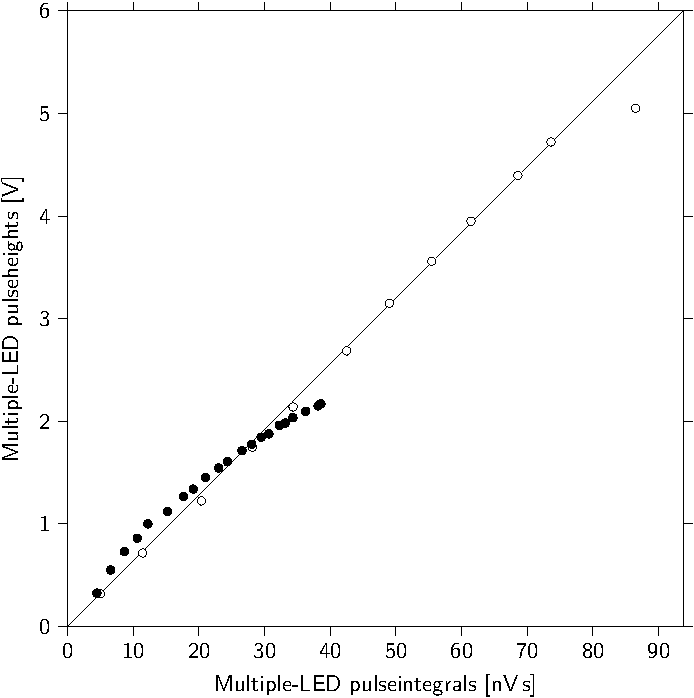
\includegraphics[width=.7\linewidth]
                    {plots/station/ph_pi_compared_nikhef_senstech}
    \caption{Measurements of the pulse height versus pulse integral. The data points show the results for the \senstech \pmt (closed circles) and the \nikhef \pmt (open circles). The last data point for the \nikhef \pmt has an unexplained offset, possibly due to a bad measurement.}
    \label{fig:ph_pi_compared_nikhef_senstech}
\end{figure}

In \cref{fig:ph_pi_503} cosmic-ray data is shown comparing a \nikhef and \senstech \pmt used in a single station. The \senstech \pmt clearly does not saturate the \adcs, while the other does. The pulse integral does continue to grow for the \nikhef \pmt while its pulse height is saturated. This is explained by the pulse becoming wider at its base. The pulse integral grows slower when some of the samples in the pulse are saturated. The difference seen in this relation for the types of \pmts can be used to identify the \pmt.

\begin{figure}
    \centering
    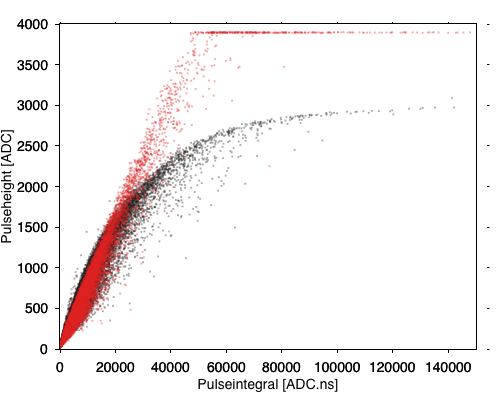
\includegraphics[width=.7\textwidth]{plots/station/ph_pi_503.png}
    \caption{Measured pulse height versus pulse integral from real detector data. The data is from detector 1 and 2 from station 503. Detector 1 (black) uses a \senstech \pmt, detector 2 (red) uses a \nikhef \pmt.}
    \label{fig:ph_pi_503}
\end{figure}

As can be seen in both the test and cosmic data, the \senstech \pmt is a bit steeper at low pulse integrals. This means that the pulses are less wide. [different number of dynodes?, different voltage?]

For each \senstech \pmt a different correction needs to be applied to the detected signals. Unfortunately, almost no \pmts have been calibrated using the LED setup. Measured cosmic data does provide some insight into the non linearity, however, the pulse height and integral are not independent measurements.

The \adcs in the \hisparc electronics are designed and calibrated to make the range \SIrange{200}{4096}{\adc} correspond to the range \SIrange{0}{-2}{\volt}. Signals greater than \SI{-2}{\volt} are clipped, preventing the pulse height to provide an accurate measure of signal strength. The pulse height clipping also affects the pulse integral. For larger signals the non-saturated parts of the signal also grow bigger, so the integral continues to increase.

In determining the particle density at a detector there are two components to look at. Given a particle density the number of particles that actually pass through a detector follows from the Poisson distribution. The width of the distribution is the square root of the mean value. This means that the error becomes larger for higher densities. Given a number of particles passing through the detector the detected signal size

- List contributions to uncertainty in particle density; Poisson, gamma's, scintillator position, pmt linearity.
- Give total uncertainty on particle density (as function of density).

Since April 2014 new \pmts are first tested in the LED setup using a single fiber to ensure it works properly. The test finds the voltage at which the output has a pulse height around \SI{340}{\milli\volt}. This pulse height value requires a voltage close to the normal operational voltage of \pmts on a \hisparc detector. The current of the \pmt is checked, high currents can indicate failing \pmts.


\section{Environmental conditions}
\label{sec:detector-environmental}

\subsection{Temperature in skibox}

LiO 2010 - Remmers - hogere T hogere MPV

The specifications of the scintillator and \pmt indicate that their efficiency depends on their temperature. The pulse height of signals determine wether they cross the thresholds in the electronics and cause a trigger. The efficiency of the detector may drop such that some events no longer cause a trigger, which they would have under normal circumstances. The change in efficiency also affects the MPV. The amount of effect the temperature has on the MPV will be examined.

About 20 \hisparc stations also have a weather station which includes a temperature sensor recording the outside temperature. The locations of the weather stations are shown in \cref{fig:weather-map}. Such enviornmental data is also available for other locations in the Netherlands from the Dutch Royal Meteorological Institute (KNMI) which operates many weather stations across the Netherlands. However, these are not at the same location as \hisparc stations. For short periods temperature probes have been placed inside the skibox, and attached to the \pmt, of some detectors to accurately measure the temperature of the detector. In \cref{fig:temperature_timeline} the values from these sensors for a month can be seen. The daily (night/day) fluctuations can clearly be seen. The skibox and \pmt temperatures clearly rise above the outside temperature. This is mostly due to the absorption of solar radiation by the skibox, and the heat generated by the \pmt. There is little to no air flow inside the skibox. On sunny days the temperatures in the skibox rise a lot higher than the outside temperature. Using solar radiation data the outside temperature can be corrected to accurately describe the skibox temperature (see \cite{devries2012weather} fig 7.7).

\begin{figure}
    \centering
    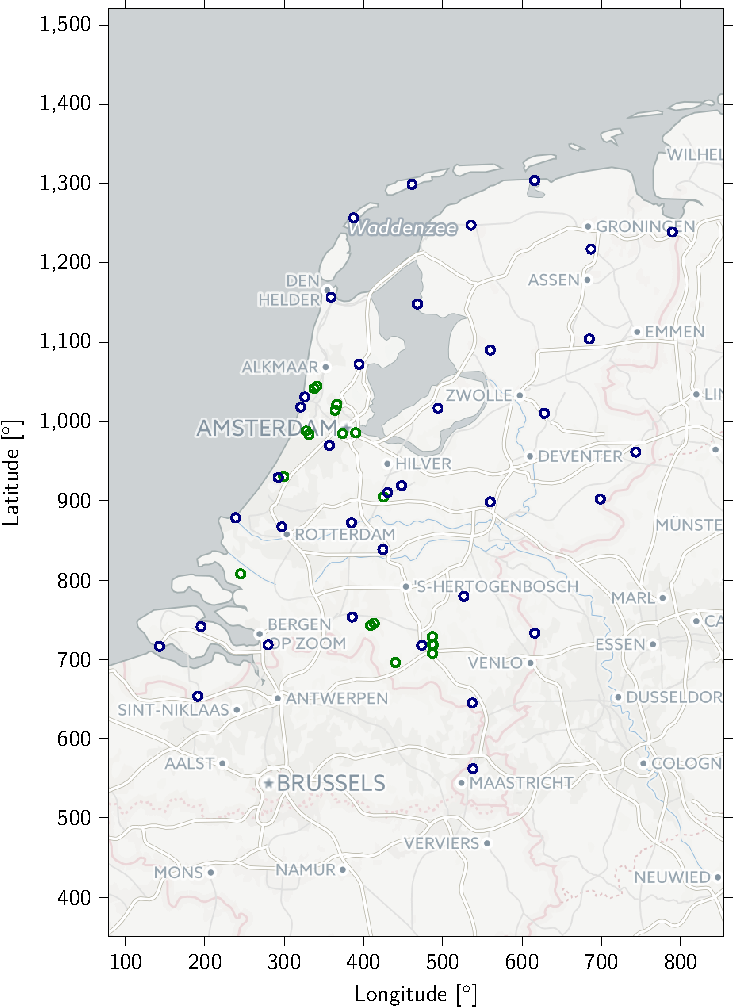
\includegraphics[width=.6\linewidth]{plots/station/weather-map}
    \caption{This map shows the locations of all \hisparc (green) and \knmi (blue) weather stations.}
    \label{fig:weather-map}
\end{figure}

\begin{figure}
    \centering
    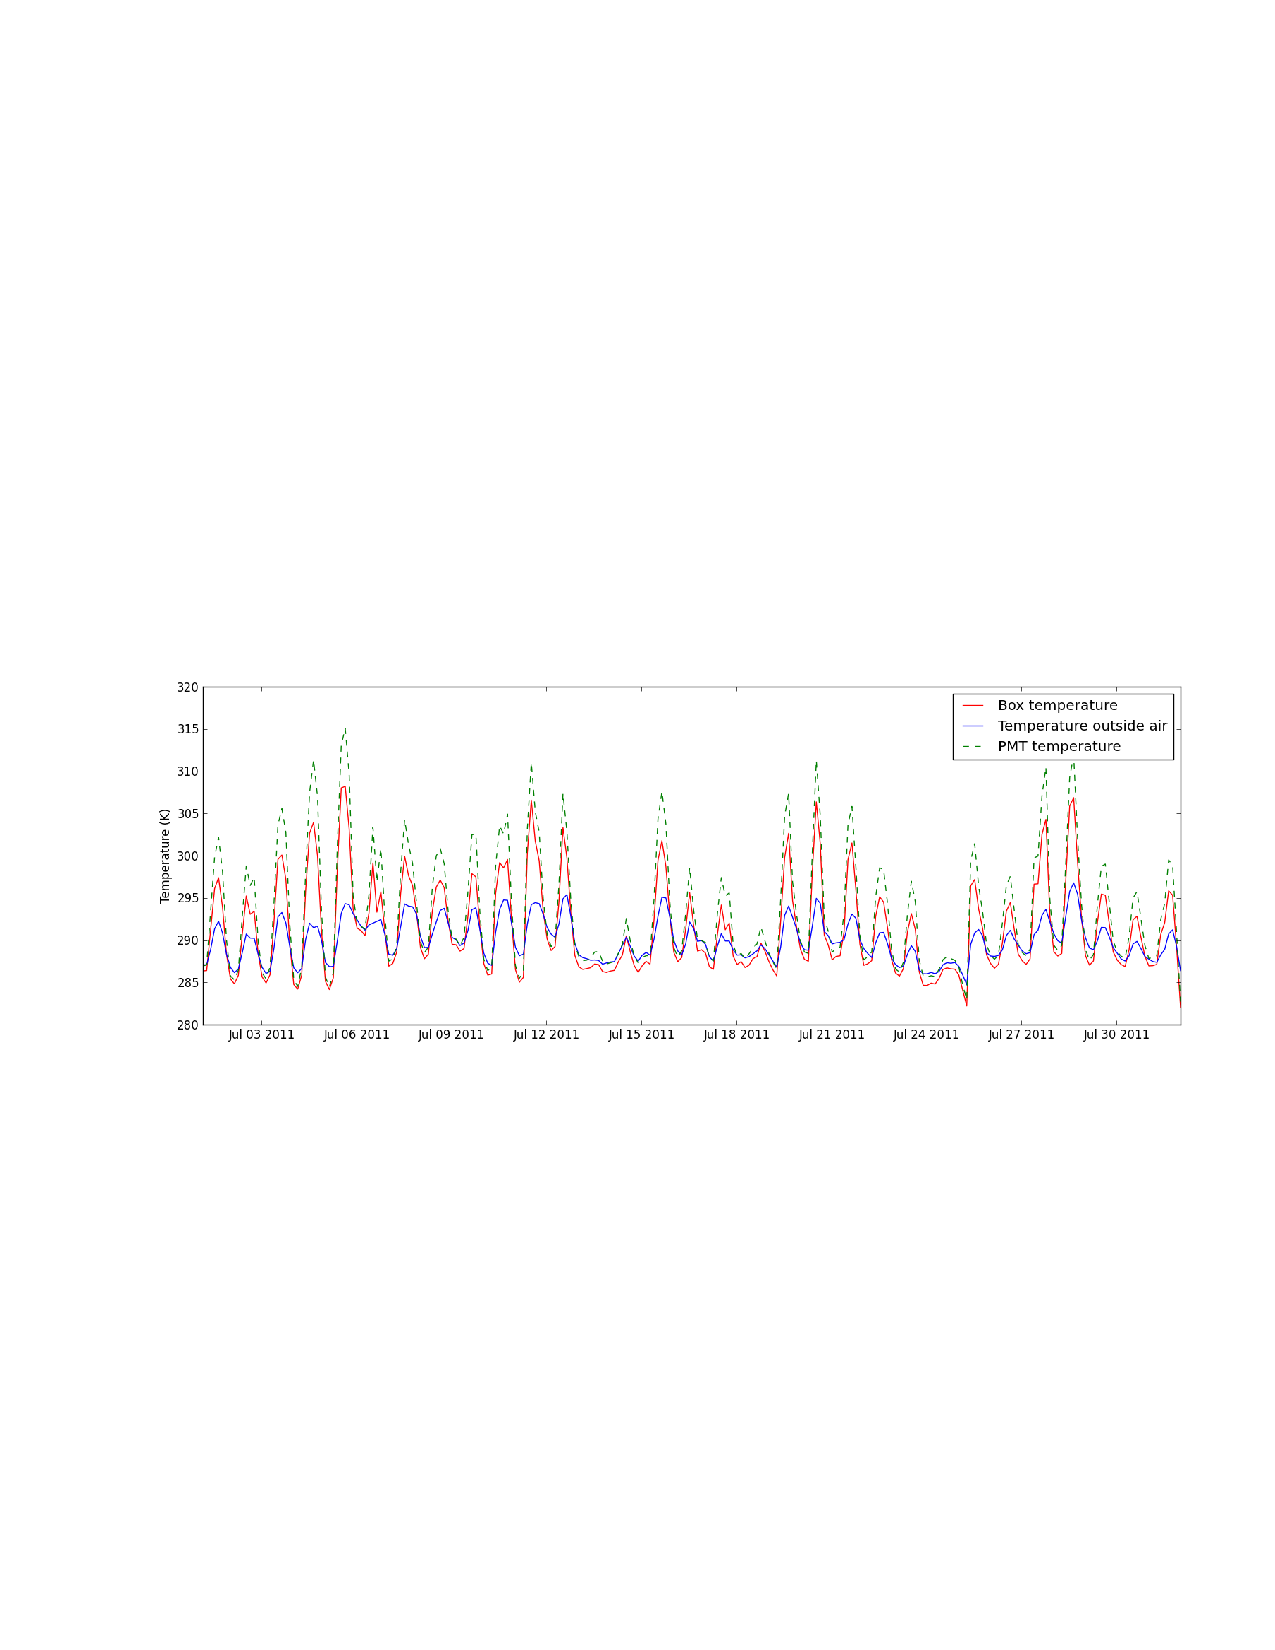
\includegraphics[width=\linewidth]{plots/station/temperature_timeline}
    \caption{Measured temperatures over time from several different sensors. A temperature probe was placed inside a \hisparc detector skibox (blue). Another sensor was attached to the \pmt of the detector (green). The weather station connected to the \hisparc station also has a temperature sensor.}
    \label{fig:temperature_timeline}
\end{figure}

A day of data is enough to accurately determine the average MPV for that day. However, daily temperature fluctuation are large enough that when the days is broken into smaller pieces different values for the MPV are found \cite{bartels2012mpv}. In \cref{fig:mpv_temperature} the reconstructed MPV is set against the \pmt temperature. The spread around the fitted line is partially caused by the temperature gradient in the periods for which the MPV is determined. The correlation agrees reasonably with the specifications of the \pmt. The specification states the gain of the \pmt changes by \SI{0.5}{\percent\per\degreeCelsius}. It does not make clear wether the efficiency increases or decreases with changing temperature, nor at which temperature it is most efficient. From our measurements it seems the gain decreases with increasing temperature. The scintillator should be \SI{100}{\percent} effective upto \SI{20}{\degreeCelsius} above which it reduces with \SI{0.125}{\percent\per\degreeCelsius}. This is but a small contribution to the reduction of the MPV. The found gradient of \SI{-0.81}{\adc\per\degreeCelsius} in the range \SIrange{200}{170}{\adc} is \SI{0.44}{\percent\per\degreeCelsius}, in close agreement with the specification. (depends on what is used as reference..)

\begin{figure}
    \centering
    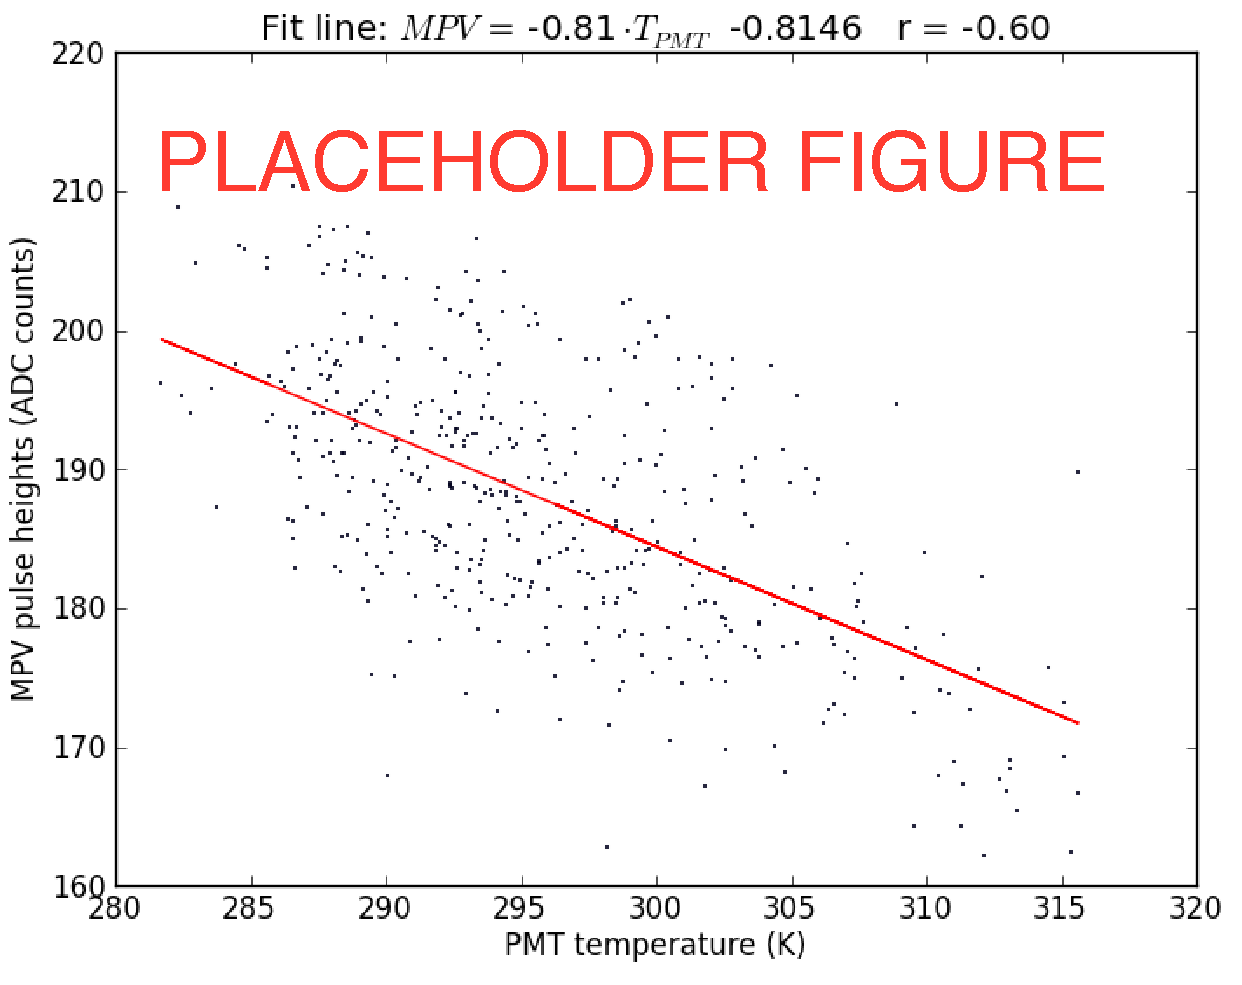
\includegraphics[width=.7\linewidth]{plots/station/mpv_temperature}
    \caption{Here we can see the correlation between the measured temperature and the MPV of the pulse heights. The red line is a linear fit to get the slope of the correlation.}
    \label{fig:mpv_temperature}
\end{figure}

Weather station data is available to correct measurements for the change in efficiency. The correction can be done using the outside temperature and solar radiation. However, this is less accurate then when the exact PMT temperature is known. Solar radiation depends on cloud cover, which may be very different from location to location depending on wind speed. Moreover, some detectors may be in the shade for parts of the day, this may mean differences of \SI{20}{\degreeCelsius} between the expected and actual temperature.


\subsection{Air pressure}

The mean free path of shower particles is determined by the thickness of the air layer it passes through. If there are more particles to collide with the chance for interaction increases. An increase in air pressure reduces the mean free path. This means more interactions in a shower. \hisparc stations are far below Xmax so the extinction processes dominate. An increase in air pressure further reduces the number of particles reaching ground level and make detection less likely.

Air pressure data is available from the \hisparc weather stations and also from KNMI data. In \cref{fig:rate_pressures} a correlation between the event rate in a station and the air pressure is shown.

\begin{figure}
    \centering
    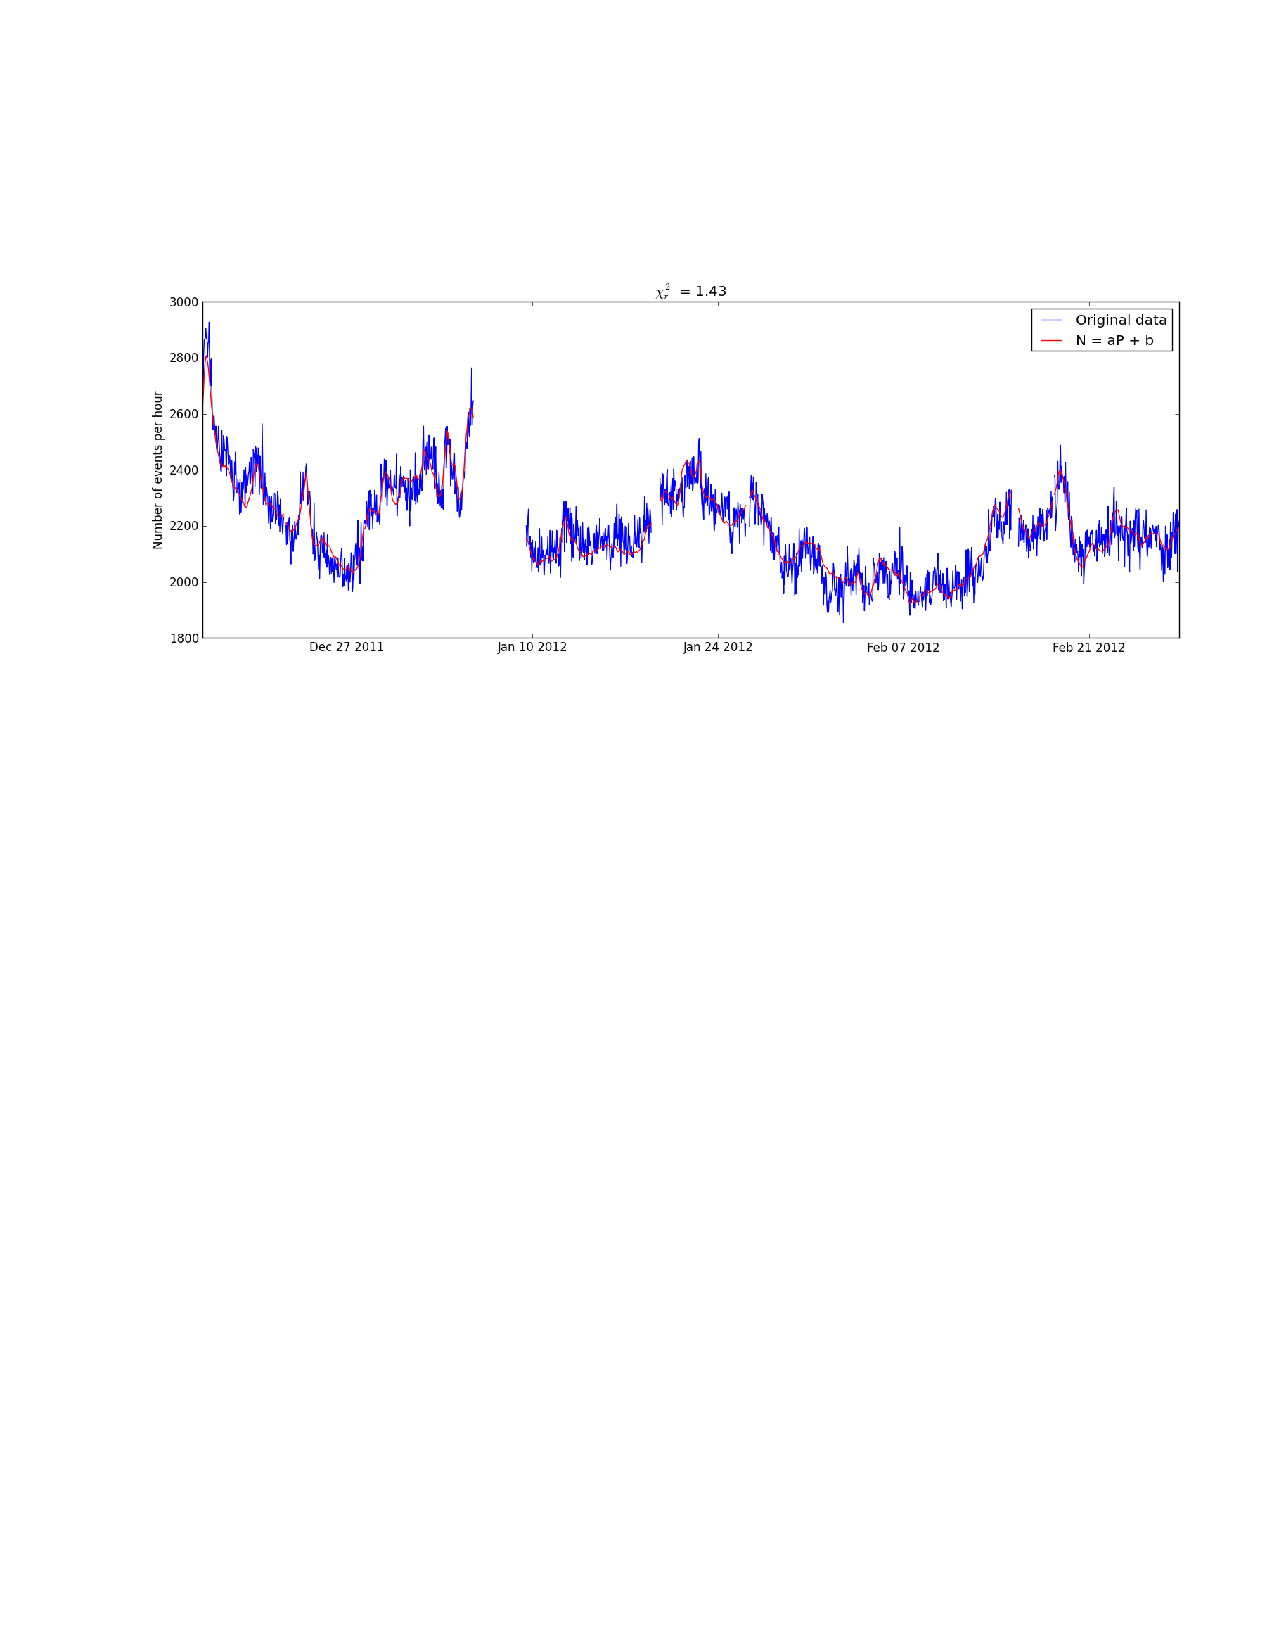
\includegraphics[width=.7\linewidth]{plots/station/barometer}
    \caption{This shows the detected number of events fitted with a model that corrects the expectation using air pressure. A better match also considers temperature. Temperature can reduce or increase signal efficiency of a detector to make trigger less/more likely.}
    \label{fig:rate_pressures}
\end{figure}

The local air pressure is to be taken into account when determining the shower energy. The relation between shower size and shower energy depends on air pressure. Air pressure does not affect the signal generated by a \mip.

[Describe how much uncertainty this adds to density reconstruction.]


\section{Durability}
\label{sec:detector-durability}

Light leaks, often directly evident after construction, some develop over time. Can be discovered in multiple ways (event rate/number of peaks). Often easy to fix by applying extra foil and tape.

The connection between the scintillator and lightguide (glue) sometimes breaks, the detector may still works but with different efficiency. As long as the detector is not moved and properly supported it can continue to operate indefinitely. Repairing the detector takes as much time as the initial construction. The glued edges needs to be sanded again.

In the small time period shown in \cref{fig:temperature_timeline} temperatures above \SI{42}{\degreeCelsius} are seen. The specifications of the \pmt state its maximum operational temperature as \SI{60}{\degreeCelsius}. Such high temperatures likely occur occasionally. However, this does not seem to be an issue.

A batch of \pmts has been encountered where the failure rate was very high, around 30 \pmts failed. This is quite a significant number since we have approximately 300 \pmts in use. The power supplies of these \pmts failed. The actual vacuum tubes were still working fine. The costs to have the power supply replaced by the manufacturer were excessive, almost equal to a new \pmt. This was one of the motivations to manufacture \pmt bases. Replacing \pmts is an easy process, this can be performed without moving the detector.

The power supplies provides by the company that assembled the HiSPARC electronics were a bad batch. They all fail within a couple months of use. These have been replaced by a different type of power supply of which no failures have been observed. Not all electronics were deployed at once, so preemptive replacements have been done for those deployed later.

On some occasions power interruptions can cause down time for a station.  There are cases where supplies were disconnected by cleaning crews or students that wanted to use the power socket for their own devices. Some schools disable their power grid during vacation time, in order to save power. Usually the station resumes operation after the vacation when the power is restored.

Despite these possible problems most detectors perform perfectly for many years, and problems can be addressed easily, as was the goal. For example station 13 on Hervormd Lyceum West in Amsterdam has been working since March 2005 with minimal interruptions. [what happened 13 august 2015?].











\section{Station}

% Impractical to connect detectors over long distances for online/realtime triggering.
By making each detection station consist of at least two detectors the station can perform triggering as a standalone unit. Each station performs its own triggering, therefore stations do not need to be interconnected. For detection stations separated by large distances this approach is more practical, since wireless and wired communication are either to unreliable or to slow. For experiments like Auger where the space between detectors is mostly empty wirelessly connecting detectors is an option. The \hisparc station consists of either 2 or 4 detectors connected to \hisparc electronics. The \hisparc electronics incorporates \pmt readout and control, triggering logic, a \gps module \cite{trimble2007resolutiont}, and a data connection to a PC. Two versions of the electronics are currently being used, versions II and III. Version III differs from II in having USB 2 (\SI{480}{\mega\bit\per\second}) instead of USB 1.1 (\SI{12}{\mega\bit\per\second}) connectors, slightly different \adcs, and an upgradable firmware over USB. The PC connected to the electronics contains software to send and receive messages to and from the \hisparc electronics. The message formats and their meaning are described in \cite{verkooijen2008firmware}, further description of the software running on the stations is described in [later chapter]. The detectors and \gps antenna \cite{trimble2015bullet} are connected to the electronics using \SI{30}{\meter} long cables.

\subsection{Signal readout}

The \hisparc electronics has two \adcs per channel, each reads the \pmt signal at \SI{200}{\mega\hertz}. By interlacing the two \adcs a sampling frequency of \SI{400}{\mega\hertz} is achieved. These are 12-bits \adcs, allowing values between \SIrange{0}{4095}{\adc} and provide approximately \SI{2}{\volt} dynamic range. The two \adcs are calibrated to provide the same baseline and gain. The baselines are set to \SI{200}{\adc} (II) and \SI{30}{\adc} (III) for the two \hisparc electronics. The two versions use a different type of \adc, with a slightly different dynamic range. The \si{\mV} to \si{\adc} conversion differs slightly, being \SI{0.57}{\adc\per\mV} (II) and \SI{0.584}{\adc\per\mV} (III). In addition to the \adcs each channel has two comparators which record the time over threshold for a given threshold. The thresholds of the comparators can be configured but are by default set to \SI{-5}{\volt} and \SI{-10}{\volt}. In case of signals which saturate the \adcs the comparators provide additional information about the actual signal size.

The \pmt signals are continually read out, the resulting \adc values are compared to two thresholds; a low and high threshold. These thresholds can be set for each channel individually. Usually they are set equally for all channels in a station, and the default setting is \SI{-30}{\milli\volt} (low) and \SI{-70}{\milli\volt} (high). The triggering logic keeps track of which channels are over a threshold and the trigger window in which trigger conditions need to be met. If a trigger occurs the time of the event is recorded as well as the trace readout of the \adc.

\subsection{Efficient triggering}

The \hisparc electronics are able to readout two detectors simultaneously. However, as mentioned stations with four detectors exist, in those cases two boxes are interconnected via UTP cables to provide readout and triggering for four detectors. When connected the two boxes still work semi-independently, but exchange threshold and \gps information. Only one of the two (the Master) contains a \gps module, it provides the second box (Slave) with \gps timing information. By exchanging threshold information the trigger logic in the Master and Slave have acces to all four channels. Triggers based on four detectors can then be created.

% Multiple detector readout with ADCs, use the good timing for coincidence time trigger.
For two detectors separated by a distance $d$ and sample rate $t_{\mathrm{sample}} = \SI{2.5}{\ns}$ the number of possible (physically relevant) time differences between the two detectors detecting the same shower front can be calculated by
%
\begin{equation}
    \begin{split}
        t_{\mathrm{max}} &= \frac{d}{c} \\
        n &= \left\lfloor \frac{t_{\mathrm{max}}}{t_{\mathrm{sample}}} \right\rfloor \\
        k &= \{x \in \mathbb{Z} : -n \leq x \leq n \} \\
        \theta_{dt} &= \arcsin \frac{k t_{\mathrm{sample}}}{t_{\mathrm{max}}} \ .
    \end{split}
\end{equation}
%
Here $\theta_{dt}$ is the set of possible angles of the shower axis relative to the line between the detectors. While placing detectors closer together increases the detection efficiency for low energy showers, it decreases the direction reconstruction accuracy.

% An efficient trigger can be made for a certain (and higher) particle density.
Using [$P_2$] we can determine the detector distance to efficiently (\SI{>50}{\percent}) detect showers as a function of primary energy. Assume the shower axis is directly between the detectors, since that is where the station will be able to most efficiently detect the shower. The following relation is plotted in \cref{fig:efficiency_distance_energy}, the transition from low efficiency to very efficient is fairly sharp.
%
\begin{equation}
\begin{split}
    r &= \frac{d}{2} \\
    P_2(d) &= \left(1 - \mathrm{e}^{-A \rho(N(E), r)} \right)^2 = 0.5 \ .
\end{split}
\end{equation}
%
So by placing the detector \SI{~10}{\meter} apart a \SI{e14.3}{\eV} shower can be detected with \SI{50}{\percent} efficiency if it fell directly between the detectors. At that distance the maximum time difference (assuming a flat shower front) between the detectors is \SI{30}{\ns}. However, shower fronts are not flat, and the rise time of the front can also cause time differences larger than expected from a horizontal shower with a flat front. Since that is a viable possibility the trigger should be long enough to also allow large time differences to detect showers when the detectors are far from the shower core.

\begin{figure}
    \centering
    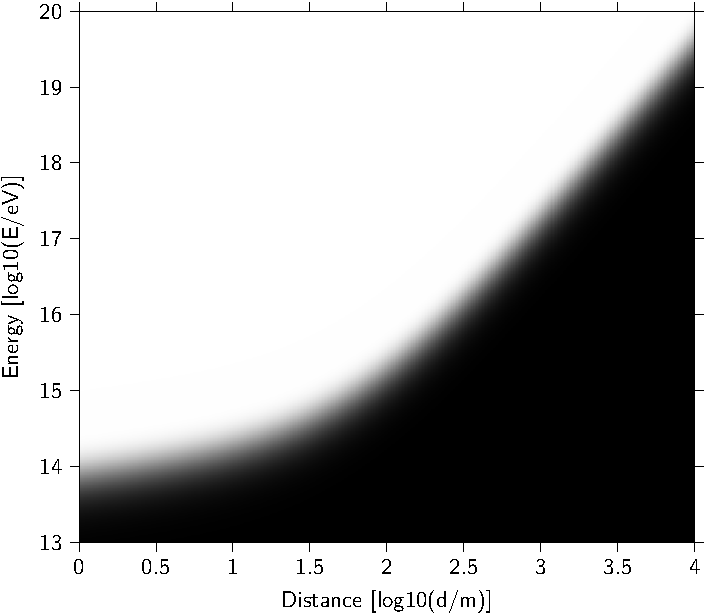
\includegraphics[width=0.6\textwidth]
                    {plots/station/efficiency_distance_energy}
    \caption{Efficiency of detection for showers of various energies as function of the distance between detectors. From impossible (black) to \SI{100}{\percent} efficienct (white). [will probably replace 2d histogram by 'contour' lines]}
    \label{fig:efficiency_distance_energy}
\end{figure}

% background rate for a given time window
In \cref{fig:temporal_profile} the temporal profile of the shower front was shown, at very large core distances the time difference between the first and last particle may be larger than \SI{3000}{\ns}. For all core distances more than \SI{50}{\percent} of the particles arrive within \SI{1500}{\ns}. This is the value that was chosen as coincidence window for \hisparc. This is long enough to account for most extreme time differences at large core distances. The number of random coincidences due to the muon background (see \cref{eq:background_rate}) with this time window is estimated to be $2 \times \SI{1500}{\ns} \times \left(\SI{0.5}{\meter\squared}\right)^2 \times \left(\SI{200}{\hertz\per\meter\squared}\right)^2 = \SI{0.03}{\hertz}$. In a properly calibrated detector the rate of singles (number of signals over the a threshold per second) are slightly higher, \SI{250}{\hertz} (low) and \SI{120}{\hertz} (high).

The standard trigger setting for a 2-detector station are 2 low signals, the high threshold is ignored. This condition has to be met within the trigger window of \SI{1500}{\ns}. This results in an event rate of approximately \SI{0.33}{\hertz}. Of which a third is expected to be from random coincidences. The low threshold is in the exponential gamma spectrum, a higher \pmt gain will increase the rate of triggers a lot, where at least one of the detectors will have a gamma.

For a 4-detector station the trigger is either 2 high signals or 3 low signals. The same trigger window is used. This results in a trigger rate of approximately \SI{0.66}{\hertz}. Of which about a fifth is expected to be due to random coincidences. The (default) layout of the 4-detector station is described in \cref{ssec:station_layout}.

% For (low energy) shower detection a station has multiple detectors close together and contains the trigger logic.
% For high energy showers the density still needs to be high enough in a station for a trigger, this limits maximum core distance for showers.
As noted, the trigger is such that low energy showers are effectively detected by the station and the time window is long enough that it can also trigger on the edges of the shower front from high energy shower.

% Using more than two detectors in a station increases detection efficiency.
% More than two detectors have the possibility of direction reconstruction.
The 4-detector station can more efficiently detect showers, since it has twice the detection area. It will trigger on lower particle densities than a 2-detector shower. This makes it capable of detecting large showers from further away. Additionally if three detectors detect a particle it might be possible to reconstruct the direction of the shower axis. This may not be accurate if the station is a the edge of the shower, because the time delays due to the rise time of the shower increase the uncertainty.

% Trigger efficiency as function of core distance and shower energy, for the different triggers (2 in 2-detector, any 2 in 4-detector, and any 3 in 4-detector for reconstructable).
The particle density threshold for triggering on showers with \SI{50}{\percent} efficiency is different for the 2- and 4-detector stations. Also an important value is the trigger efficiency for at least 3-detectors with a hit in the 4-detector station, since this can result in reconstructable showers. In \cref{fig:ldf_energies2} the energy which can be triggered with \SI{50}{\percent} efficiency as a function of core distance is shown for these three cases.

\begin{figure}
    \centering
    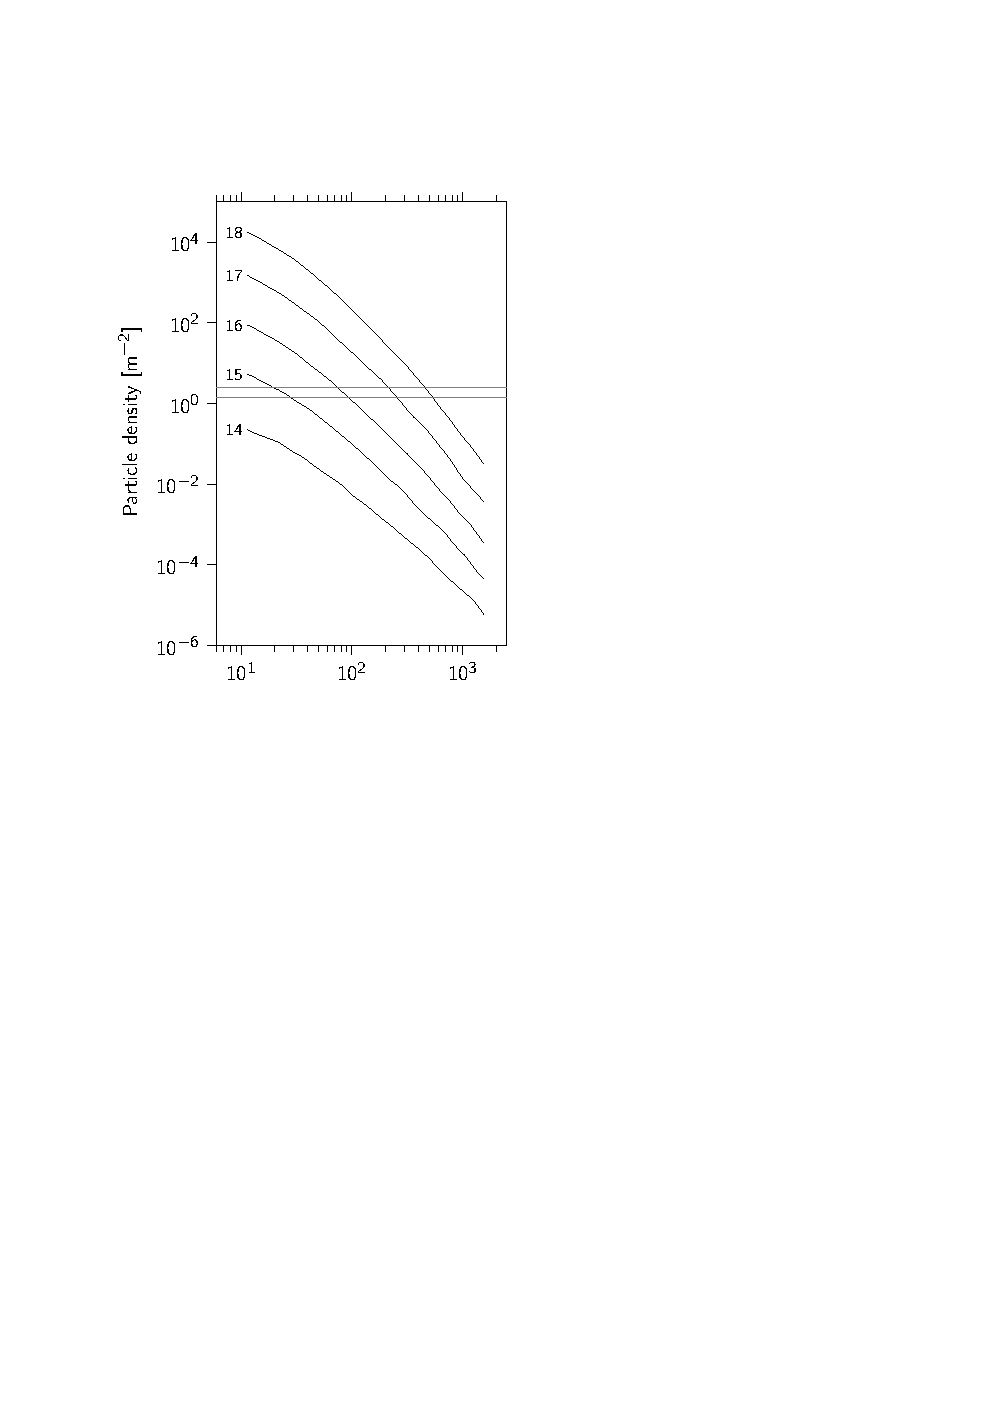
\includegraphics[width=0.5\textwidth]
                    {plots/station/ldf_energies}
    \caption{Trigger efficiency E = \SIrange{e14}{e20}{\eV} showers, add horizontal lines for 2 in 2-detector, any 2 in 4-detector, and any 3 in 4-detector (\SI{50}{\percent} efficient.}
    \label{fig:ldf_energies2}
\end{figure}

\begin{figure}
    \centering
    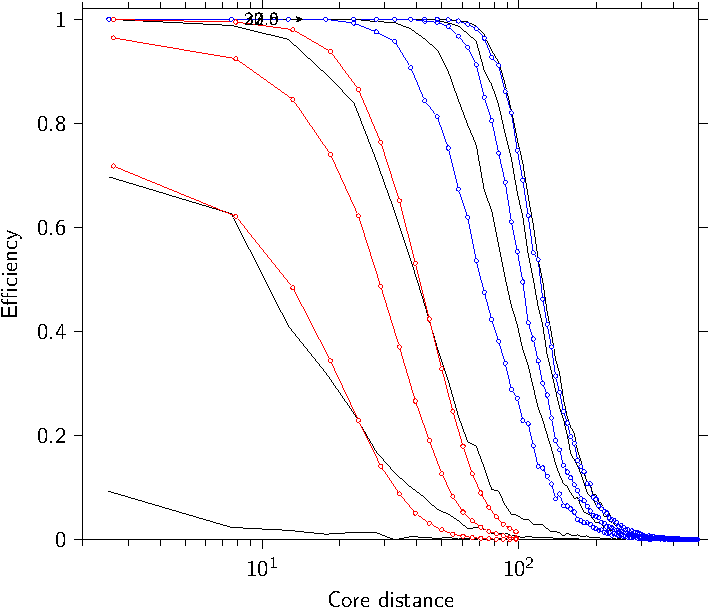
\includegraphics[width=0.6\textwidth]
                    {plots/station/efficiency_two_16}
    \caption{Detection (trigger) efficiency as a function of core distance for showers of different primary energy (and zenith).}
    \label{fig:efficiency_two_16}
\end{figure}

% Explain simple direction reconstruction with 3 detection points (flat/curved shower).
When there are three detection points which are not on a line the shower axis can be constrained. In this case the detectors are assumed to be at the same height and the front is considered flat, an approximation which can be valid at the short distances between detectors as they occur in a station. The 2-dimensional flat-front reconstruction method for three detection points is described in \cite{fokkema2012hisparc}. The following equations result in the shower axis direction, i.e. the azimuth ($\phi$) and zenith ($\theta$).

\begin{equation}
    \label{eq:direction-2dflat}
    \begin{split}
        \phi &= \arctan \left(\frac{r_1 \Delta t_2 \cos \phi_1 - r_2 \Delta t_1 \cos \phi_2}{r_2 \Delta t_1 \sin \phi_2 - r_1 \Delta t_2 \sin \phi_1} \right) \ , \\
        \theta &= \arcsin \left(\frac{c \Delta t_i}{r_i \cos(\phi - \phi_i)} \right) \ .
    \end{split}
\end{equation}

Here $r_i$ is the distance between detector 0 and detector $i$, $\Delta t_i$ is the time difference between detector 0 and detector $i$, and $\phi_1$ the angle between East and detector $i$ as seen from detector 0. Note that care must be taken to take the correct quadrant for the $\arctan$ and that $\phi - \phi_i \ne 2 \pi$. The same results can be achieved with a Cartesian approach as described in \cite{montanus2015direction}. This gives

\begin{equation}
    \label{eq:direction-2dflat}
    \begin{split}
        \phi &= \arctan \left(\frac{-u_x v_z}{u_y v_z} \right) \ , \\
        \theta &= \arcsin \left(\sqrt{\frac{u_x^2+u_y^2}{v_z^2}} \right) \ .
    \end{split}
\end{equation}

Here $u_x = \Delta t_2 x_1 - \Delta t_1 x_2$, $u_y = \Delta t_2 y_1 - \Delta t_1 y_2$, and $v_z = x_1 y_2 - x_2 y_1$. The $x$ and $y$ coordinates are as defined by the ENU coordinate system described in [ref apprendix coordinates], in this case using detector 0 as reference.

\subsection{Station layout}
\label{ssec:station_layout}

% Standard layouts created to encourage uniformity, these are also chosen for good shower acceptance, reconstruction accuracy of station events, and practicality for the locations.
The layouts of a typical 4-detector station is shown in \cref{fig:4_detector_layouts}. The detectors are separated by \SI{10}{\meter} to exclude the smallest showers and provide accurate direction reconstruction resolution. Given the location of the station is on the roofs of buildings the size of typical roofs also limits the possible size of the stations. The distance between detectors also affects the resolution for reconstructing the direction of air showers. The possible directions for three detectors in an equilateral triangle with \SI{10}{\meter} sides and a timing resolution of \SI{2.5}{\ns} is shown in \cref{fig:discrete_directions}. Using the inner detector with two outer detectors reduces the direction resolution, having only 1/3rd the possible directions. In some cases (space allowing) the decision has been made to move the inner detector outside the triangle to form a second equilateral triangle sharing one of the sides. In this case all combinations of three detectors result in the same possible direction reconstructions.

\begin{figure}
    \centering
    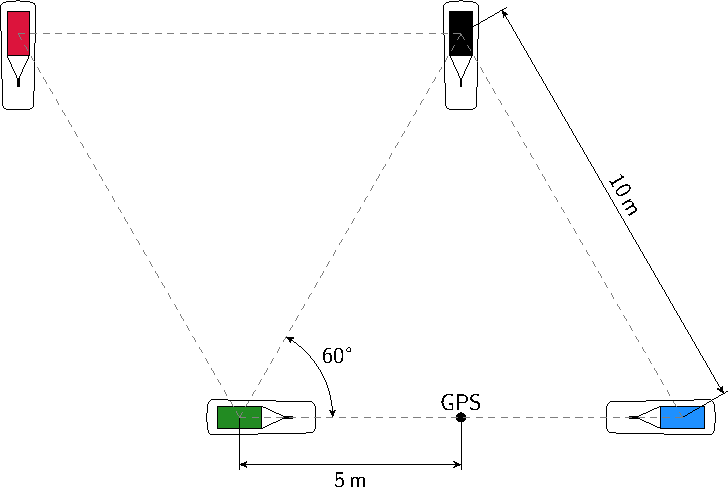
\includegraphics[width=0.4\textwidth]
                    {plots/station/4_detector_diamond}
    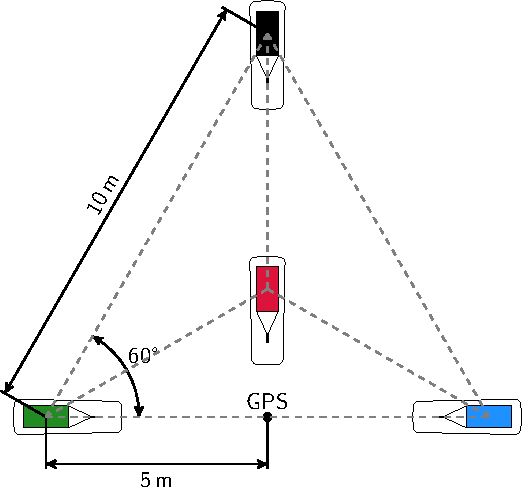
\includegraphics[width=0.4\textwidth]
                    {plots/station/4_detector_star}
    \caption{4-detector station layouts. 4-detector stations are typically placed in the diamond or star formation. Both contain multiple triangles between sets of 3 detectors.}
    \label{fig:4_detector_layouts}
\end{figure}

\begin{figure}
    \centering
    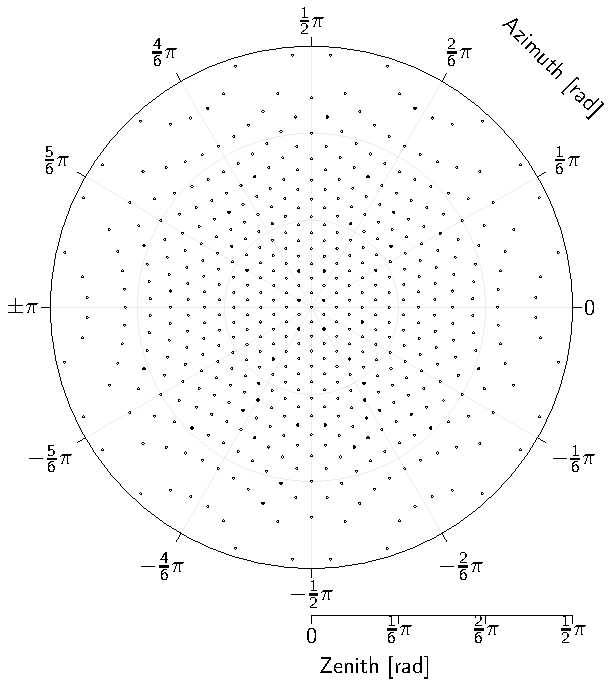
\includegraphics[width=0.6\textwidth]
                    {plots/station/discrete_directions}
    \caption{Both 4-detector layouts result in the following distribution of possible shower directions given \SI{2.5}{\ns} arrival time sampling in the detectors. For the diamond layout more points can be made by more combinations, i.e. more possible solutions. Approximately \SI{5}{\degree} between adjacent points near Zenith.}
    \label{fig:discrete_directions}
\end{figure}

The layout of each station is not always precisely according to the suggested layout. Not all roofs provide the required space. It is not a problem if the layout deviates from the suggested ones, as long as the actual positions are known. In order to get the absolute position of the detectors their positions are measured relative to the \gps antenna, whose position is know. From the \gps the distance to and the angle between (True?) North and the detector (the center of the scintillator) is measured. Additionally the rotation of the detector itself around its center can be recorded, though this is less important. The coordinate system is also described in \cref{ch:coordinates}. If the location of detectors relative to the \gps is changed the new layout can be recorded with the timestamp of when it changed. The data analysis takes these changes into account to use the correct layout when reconstructing events. For students a document has been created which outlines the steps for measuring their detector positions and how they can submit them to the Public Database. Information about the position of detectors in 2-detector stations is also important. Though full direction reconstruction is not possible with only two detectors it can define a plane where the shower should come from (reference Niek).

\subsection{Reconstruction accuracy}

The reconstruction accuracy of a single \hisparc station was tested at the \kascade experiment. The \hisparc station was placed between the \kascade detectors and triggered (using an external trigger) when the surrounding detectors detected an event. The \kascade reconstruction of the events which triggered the \hisparc station were made available. By applying the reconstruction to the data and comparing this to the \kascade reconstruction the performance of a single station is tested.

The reconstruction of the shower direction has shown to be accurately reconstructable. The results reported in [ref fokkema] are shown in \cref{fig:azimuth_kascade_minn1}.

\begin{figure}
    \centering
    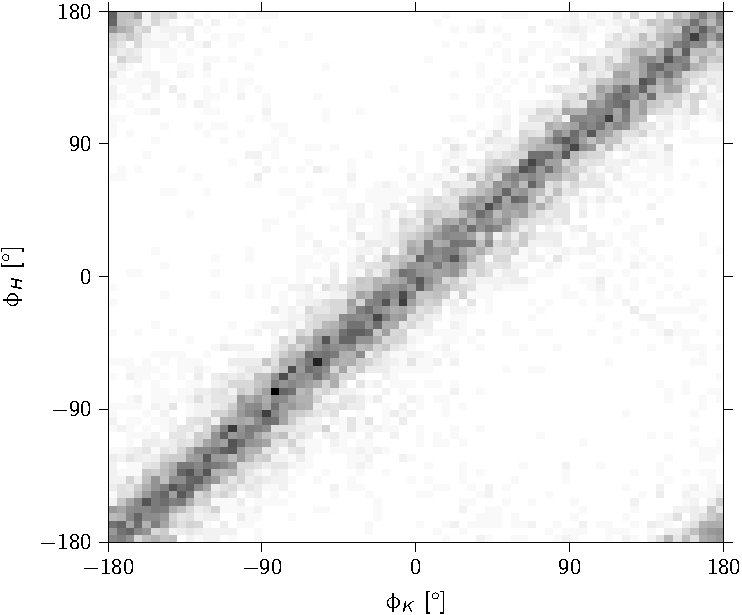
\includegraphics[width=0.6\textwidth]
                    {plots/station/azimuth_kascade_minn1}
    \caption{Test station at KASCADE was used to verify the performance of a single station. The direction agreement between simultaneously detected events is shown.}
    \label{fig:azimuth_kascade_minn1}
\end{figure}

% Shower core/energy determination impractical with single station.
Determination of the shower core is impractical with a single station. The error on the determination of the particle density is to high and the number of detection points to low. In \cref{fig:n_501_510_sum} the predicted (by \kascade) particle density at a detector is compared to the actual measured signal. The large spread is due to the Poison, Landau, transmission, and \pmt gain distributions.

\begin{figure}
    \centering
    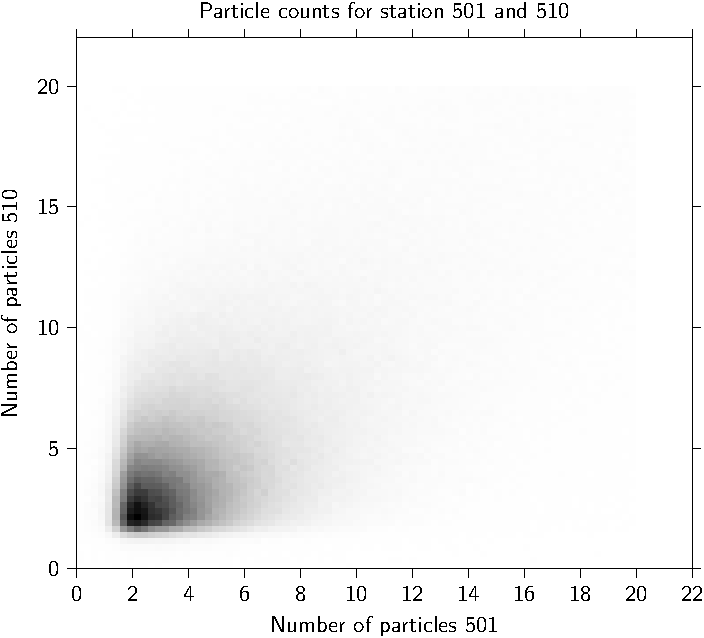
\includegraphics[width=0.6\textwidth]
                    {plots/station/n_501_510_sum}
    \caption{(place holder figure showing different data) Test station at KASCADE used to verify the particle density measurement of a single detector and full station, compared to the KASCADE predicted particle density.}
    \label{fig:n_501_510_sum}
\end{figure}


\subsection{Weather station}

% Optional weather station to provide local weather data.
Optionally a \hisparc station can be extended with a weather station to provide local weather measurements. These measurements can help in understanding how shower development is affected by atmospheric conditions. For instance an high air pressure increases the number of collisions in air showers, thereby reducing the number of particles that reach sea level. This lowers the trigger rate for a station. Additionally some of the detector components have efficiencies dependent on their temperature. By measuring the temperature detections may be corrected for the changed efficiency. \hisparc uses a Davis Vantage Pro 2 weather station \cite{davis2012vantagepro} which includes the following sensors; temperature, relative humidity, atmospheric pressure, wind direction, wind speed, solar radiation, UV index and rain rate. These sensors are readout at a \SI{5}{\second} interval. Currently there are 19 \hisparc stations that also have a weather station. These locations are shown on the map in \cref{fig:map_weather_knmi}.

\begin{figure}
    \centering
    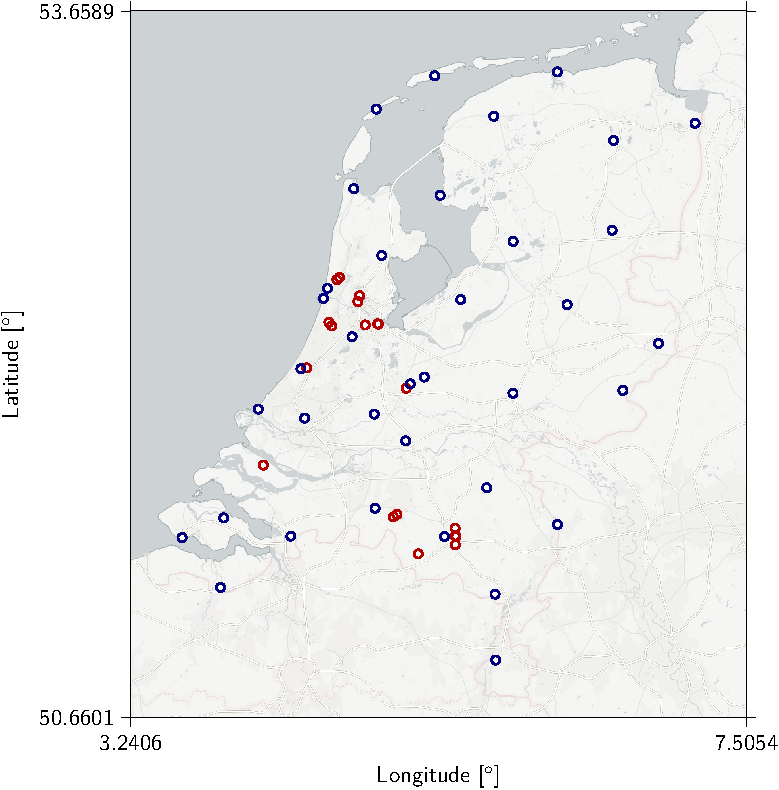
\includegraphics[width=0.6\textwidth]
                    {plots/station/map_weather_knmi}
    \caption{Locations of HiSPARC weather stations (red) and the KNMI weather stations (blue).}
    \label{fig:map_weather_knmi}
\end{figure}

% May not be required at each station, can use freely available KNMI data. However, in some cases closest KNMI station is far away.
Note that it is not required for all stations to have a weather station. The Royal Dutch Meteorological Institute (KNMI) also provides a public weather data service in the Netherlands. KNMI has 36 stations spread in a regular grid around the Netherlands. Not all \hisparc stations are close to a KNMI station, for some weather quantities this is no problem because they are similar over long distances, or can be interpolated. Besides temperature the local solar radiation strongly influences the temperature of the detector in a ski-box.






\section{Signal digitization}

The signal in one channel is sampled by two \adcs. To get good data and triggering the \adcs need to be calibrated to have the same baseline and response (gain). The \adcs normally have a range of \SIrange{-1}{1}{\volt} translated into a 12-bit value. This is good for AC signals, but the \pmt outputs negative pulses. Any positive pulses are less important, but can be used to detect reflections. An electric circuit in the \hisparc electronics modifies the incoming signal to increase the dynamic range for the DC pulses. The baseline of the signals is calibrated to make an input of \SI{0}{\volt} correspond to \SI{200}{\adc} (\hisparcii) or \SI{30}{\adc} (\hisparciii). The gain is such to get a conversion factor of \SI{-0.57}{\milli\volt\per\adc} (\hisparcii) or \SI{-0.584}{\milli\volt\per\adc} (\hisparciii). This results in an effective range of \SIrange{-2.222}{0.113}{\volt} (\hisparcii) or \SIrange{-2.374}{0.018}{\volt} (\hisparciii).

The two thresholds used for the trigger are \SI{-30}{\milli\volt} (low) and  \SI{-70}{\milli\volt} (high). These correspond to \SI{53}{\adc} (\hisparcii) or \SI{50}{\adc} (\hisparciii), and \SI{123}{\adc} (\hisparcii) or \SI{120}{\adc} (\hisparciii) above the baselines. However, for some stations slightly different threshold may be used, the chosen thresholds are sent to the datastore as part of the station configuration. In the data processing the thresholds from the configuration data need to be used for trigger time reconstruction.


\subsection{\adc sampling}

The \pmt signals are sampled every \SI{2.5}{\ns} alternately by the two \adcs.
In order to get consistent data both \adcs are aligned to have the same baseline and gain. \adcs remain accurate when they have a constant temperature. When \hisparc electronics are first connected the temperature will likely be below operating temperature. When calibration is performed immediately after powering the electronics it may drift from proper calibration as it continues to operate [how much drift?]. An offline/software based Mean Filter [ref to later section] in the software is capable of smoothing the combined signal. This removes any small misalignment effects. Slightly different gains can cause very bad alignment at higher voltages. An example of misaligned traces is shown in \cref{fig:adc_alignment}.

\begin{figure}
    \centering
    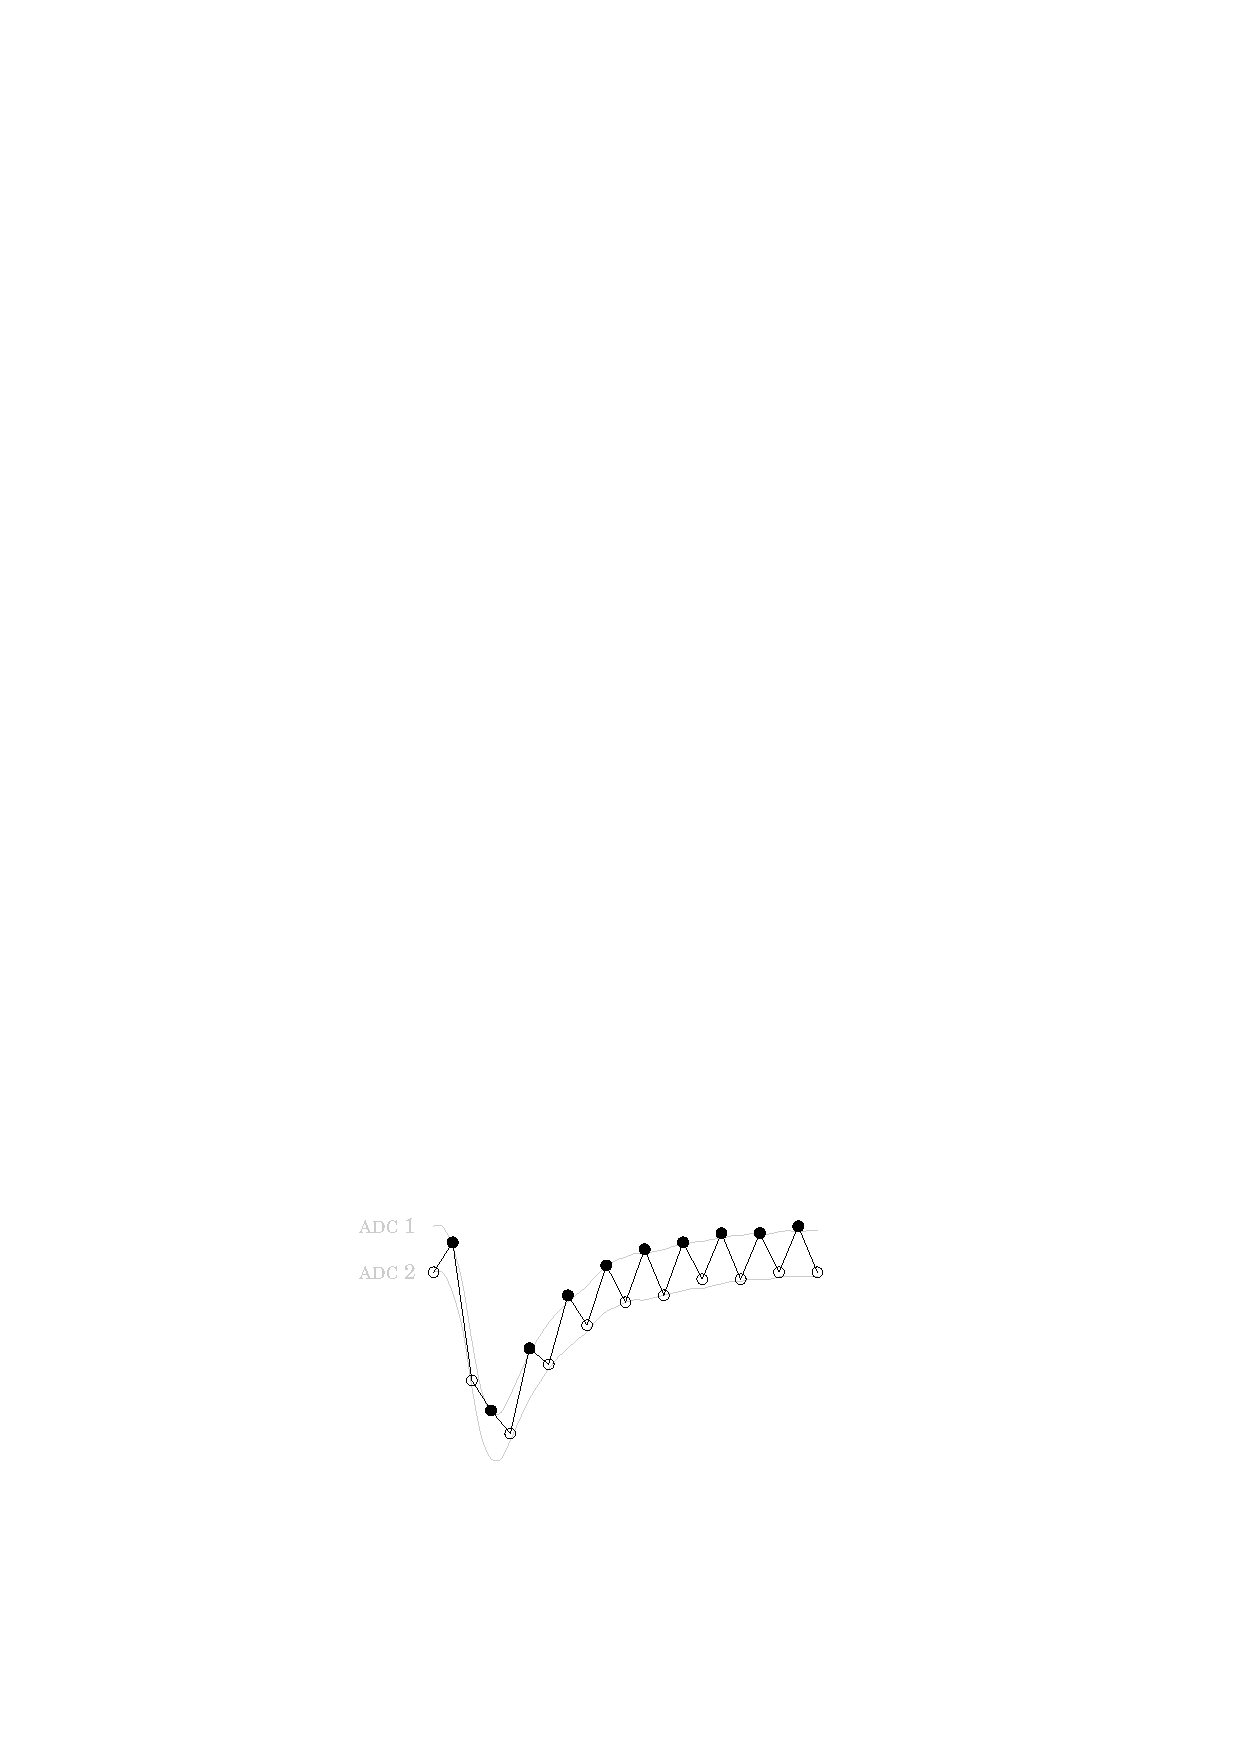
\includegraphics{plots/station/adc_alignment}
    \caption{Signals are read by two \adcs alternatively (open and closed circles). When the \adcs are not properly aligned they return different results for the same input.}
    \label{fig:adc_alignment}
\end{figure}


\subsection{Comparators}

LiO 2011 - Marcelis?

The non-linearity of the \pmt response described in the previous chapter means that many \pmts will never saturate the \adcs. The \hisparc electronics also includes two comparators per channel which determine if a signal reaches two higher thresholds (\SIrange{2}{10}{\volt}). These will remain unused with most stations. For the new \pmts the comparators will be essential in signal reconstruction of high particle densities. However, the readout of the comparators was not implemented in the software until the end of 2015. So these will not be taken into further account in this thesis.


\section{Timing}


\subsection{Trigger time and the Mean Filter}

An additional effect of misalignment is the probability of either \adc being the one which causes a trigger. An \adc with a slightly higher baseline (in \adc counts) is more likely to cause a trigger. This effect is reduced when looking at events with higher particles densities because the rise time of the pulses is reduced. (or steepness of pulse front is higher). This can be seen in [figure with histogram of trigger time], the reconstructed trigger time has a preference for one of the two channels. The preference matches the ADC which has a higher baseline.

In the DAQ software used before 2016 activating the Mean Filter would also apply the filter on the traces being sent to the datastore. This is not desirable because the reconstruction of the trigger time in the event requires unfiltered traces. However, in most cases trigger reconstruction will be successful on filtered traces, unless the pulse heights are very close to the thresholds used in the trigger. In that case the filter may reduce the signal to values below the threshold making reconstruction impossible, since the filter is destructive/irreversible.


\subsection{Mean Filter and trigger reconstruction}

The misalignment of the \adcs also affects the arrival time reconstruction. However, to reduce the preference for either \adc the mean filter can be applied to unfiltered traces before reconstructing arrival times.

- Rise time effect on arrival time reconstruction.


\subsection{Detector offset calibration}

- [figure] arrival time distribution between two detectors in a station
  Detector offsets can be determined with a day of data (accuracy?). Arrival
  time differences give an almost Guassian distribution.

The offsets between detectors in a station can be very stable over time. Changes to the station hardware and configuration can distrupt this. In \cref{fig:detector_offset_drift_month_501} the detector offsets for station 501 are shown. The jumps in offsets are explained by the change to \hisparciii electronics.

\begin{figure}
    \centering
    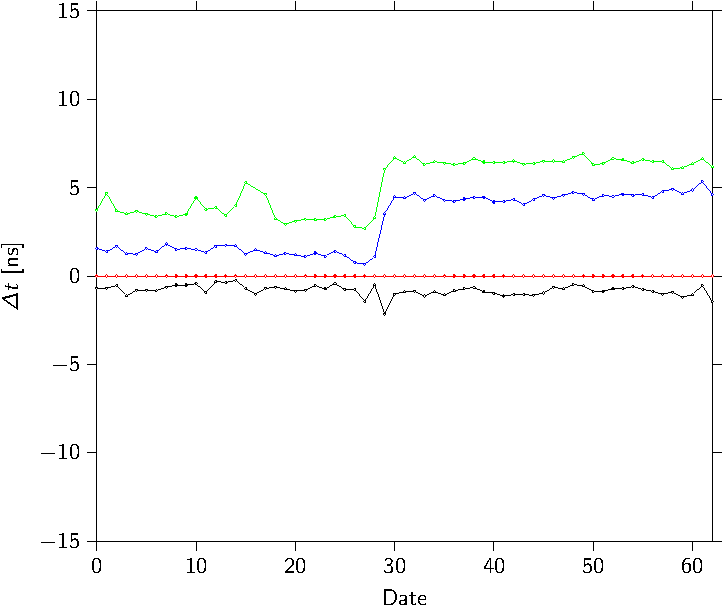
\includegraphics{plots/station/detector_offset_drift_month_501}
    \caption{This shows the changes in detector offsets for the detectors of station 501. Detector two is used as reference. The large jump observed for detector 3 (green) and 4 (blue) was caused by the use of \hisparciii electronics.}
    \label{fig:detector_offset_drift_month_501}
\end{figure}

These detector offsets are automatically determined each day for each station. In \cref{fig:detector_offset_distribution} the distribution of the offset between the two detectors connected to the Master electronics is shown. The mean offset is $0.02 \pm 0.30 \si{\ns}$ and the width of the distribution is $2.31 \pm 0.24 \si{\ns}$. The distribution between Master and Slave is more offset with a mean of $1.00 \pm 0.60 \si{\ns}$ with approximately the same width $2.25 \pm 0.84 \si{\ns}$.

\begin{figure}
    \centering
    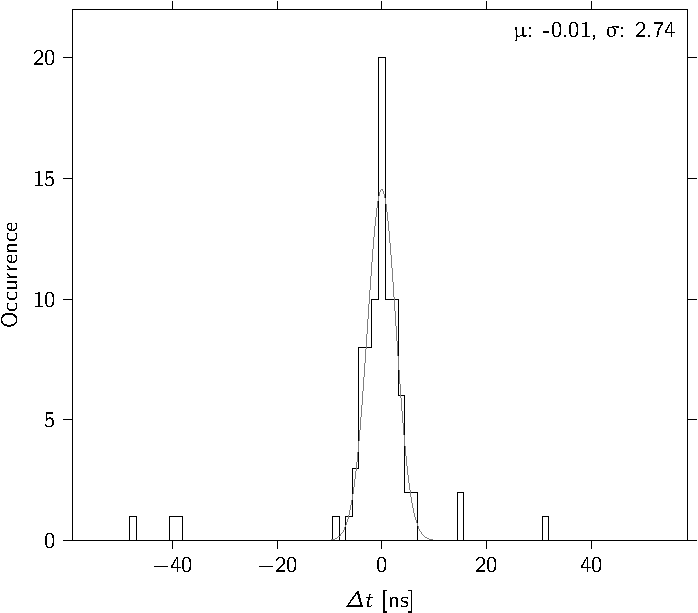
\includegraphics{plots/station/detector_offset_distribution}
    \caption{Distribution of detector offsets. The detector offsets between the two detectors connected to the Master electronics for all \hisparc stations are shown.}
    \label{fig:detector_offset_distribution}
\end{figure}

Clearly the offsets are often very small, with some outliers.

- [figure] distribution of detector offsets between master and slave
  [figure] time delta distribution (depends on trigger slave/master?)


\begin{figure}
    \centering
    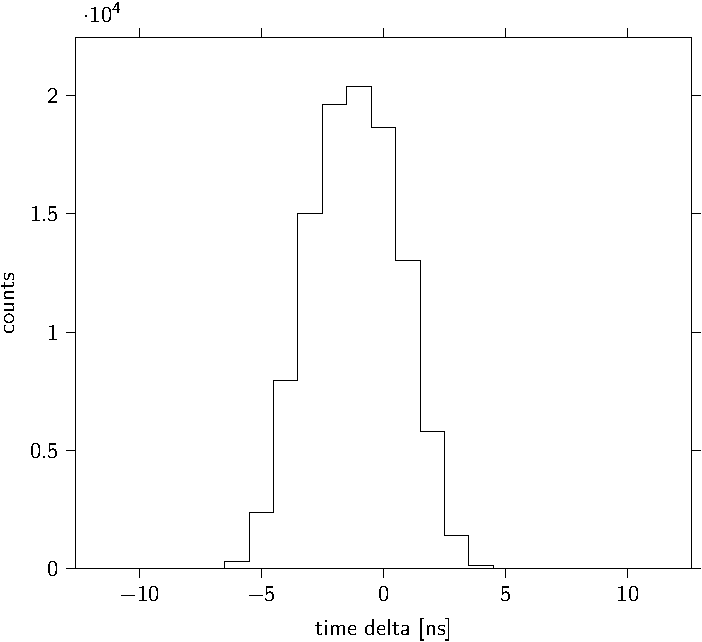
\includegraphics{plots/station/time_delta_501}
    \caption{.}
    \label{fig:time_delta_501}
\end{figure}


The Master and Slave determine their own timestamp for events. The difference between these timestamps is not stored, it is only used to find events that belong together on the station PC. The overal offset between master/slave is corrected for by correcting for detector offsets, small error remains.


\section{Station layouts}

Not all station locations are able to fit the suggested layouts. So slightly modified versions exist. Moreover, not every station is angled the same way relative to North. The detector locations are essential for direction reconstruction, if the angle of a station is not known the reconstructed directions will point to the wrong place on the sky.

\gps positions are automatically submitted by the station to the datastore. Detector positions are not measured automatically, so they need to be measured by hand. Since the \gps antenna position is known, the detector positions relative to the \gps are desired. The coordinate system used to describe detector positions is described in \cref{ch:coordinates}. Moreover, in some stations detectors have been moved into a new configuration, sometimes more than once. Each time the detector positions relative to the then-current position of the \gps need to be determined, including the time of the change. Only if relative position of \gps and detectors change must a new position be submitted. Station supervisors can submit their measured layout, which will be reviewed by one of the \hisparc coordinators. Satellite imagery can sometimes be used to verify the positions of the detectors. These variable detector and \gps positions are taken into account when reconstructing showers.

In \cref{fig:locations_501} the different \gps and detector locations for station 501 are shown. The outlier \gps locations are caused by the usage of temporary \gps antenna during tests. The station layout described by the clustered positions describes the original star-layout, an equilateral triangle with one detector in the center. When station 510 was built station 501 was also moved to create overlapping diamond-shaped stations. Detector 3 (green) was not moved during this transition. For each physical \gps location (including the temporary test locations) the relative detector positions have been measured. Other Science Park stations for which the detectors have been moved are 502 and 505. For station 505 this was done multiple times because alterations to the roof on which the detector reside required them to be moved.

\begin{figure}
    \centering
    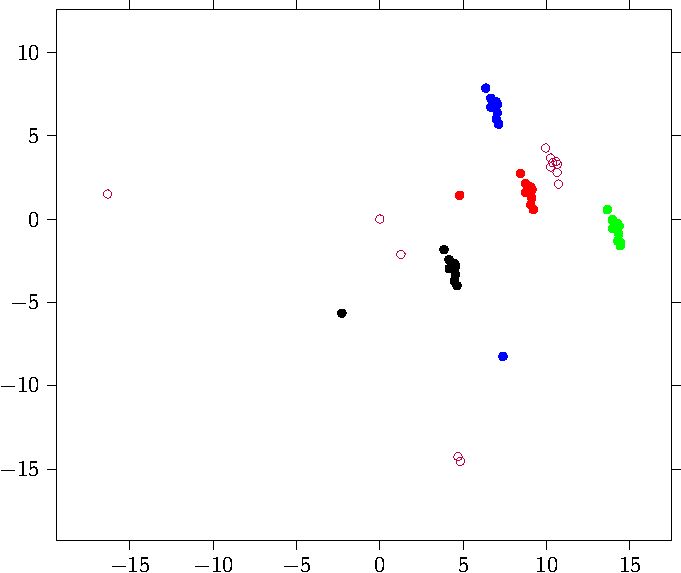
\includegraphics{plots/station/locations_501}
    \caption{Detector (closed circles) and \gps locations (open circles) for station 501. Over time the detectors and \gps antenna for station 501 have been moved multiple times. The large clusters of circles are not necessarily movement of the \gps and detectors but merely new self-surveys by the \gps resulting in a slightly different position.}
    \label{fig:locations_501}
\end{figure}


\section{Overlapping stations}

Station 510 was created to overlap with station 501. Because of the nearly identical detector positions the stations often detect the same showers. Because of this the trigger efficiency and reconstruction accuracy between the two can be compared. These stations work independently, like other stations.


\subsection{Detection efficiency}

The detection efficiency is defined as the probability of a detection given a certain event/particle density. This is determined by checking if the stations are in coincidence or not. For all events in a particle density bin for one station the number of simultaneous events in the other station is counted. These values are then divided to get the probability of an event in the other station given a particle density. In this case we do not know the exact particle density and the station used as reference is also affected by its own detection effciency. So in fact the efficiency of both stations is combined. In \cref{fig:effiency_501_510} the detection(/coincidence?) effiency for 501 (solid) and 510 (dashed) are shown, given a particle density in the other station.

\begin{figure}
    \centering
    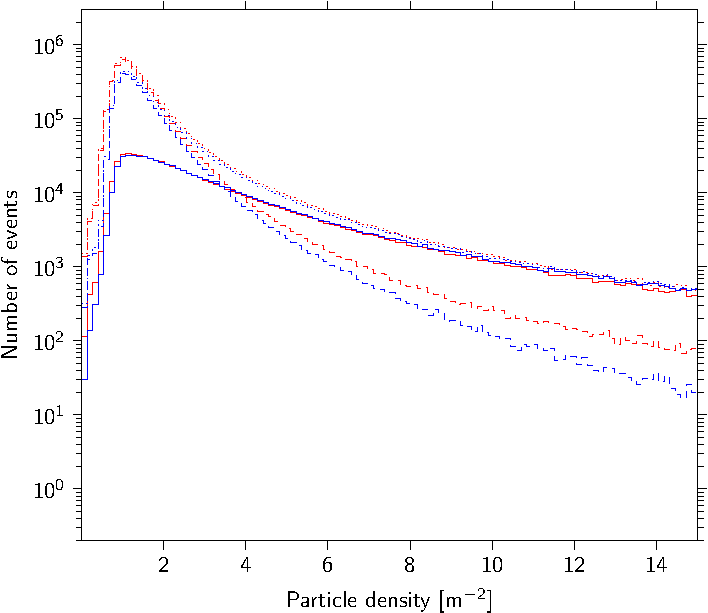
\includegraphics{plots/station/anti_coincidences}
    \caption{Detection efficiency in stations 501 (solid) and 510 (dashed) versus the density measured by the other station. TODO: new plot, currently divide solid by dotted to get effiency.}
    \label{fig:effiency_501_510}
\end{figure}

At a particle density of approximately \SI{3.5}{\per\square\meter} in one station the coincidence probability for the other station becomes \SI{50}{\percent}. At approximately \SI{2.2}{\per\square\meter} the detection probability becomes \SI{25}{\percent}.

[todo P{501+510}, P{501+!510}, P{!501+510}, P{!501+!510}]

For the events in coincidence we can compare how well the two stations sampled the shower, and how well the detections can be reconstructed. In \cref{fig:density_501_510} the density correlation between the possible combinations of detectors is shown. The pairs of adjacent detectors form the diagonal. A stronger correlation can be seen for the detectors which are close together. Detectors 1 and 3 are furthest appart, resulting in the wider distribution.

[todo width explained by Poisson/signal transport distribution]

The effects of \pmt linearity can be seen. Station 510 uses \nikhef \pmts. Consequently, for higher particle densities the average pulse integral for 510 will be higher. This is why the histograms are not more symertrical around $x = y$.

\begin{figure}
    \centering
    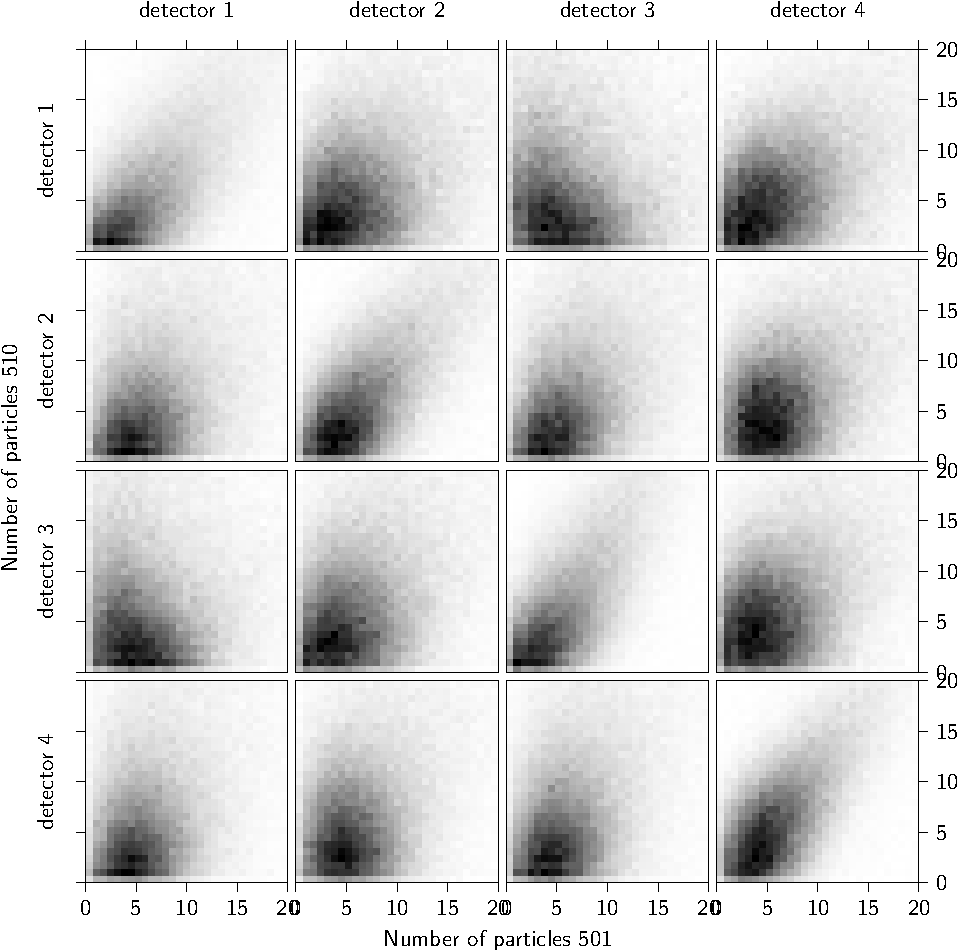
\includegraphics{plots/station/n_minn16_501_510_bins}
    \caption{Particle density correlation in detectors for events in coincidence between 501 and 510.}
    \label{fig:density_501_510}
\end{figure}


\subsection{Reconstruction accuracy}

For events in coincidence the direction reconstructions (arrival time gradients?) can be compared to see the distance between the reconstructions. For events with higher particle counts the direction reconstruction accuracy increases. This is because of several reasons. First, the probability of detecting a particle from the front of the shower front increases. Secondly, increased probability that a particle hits the detector close to the \pmt, reducing the transport time. Thirdly, the rise time of the signal decreases. Fourthly, the increased particle density increases the probability of being close to the shower core, where the shower front is more flat, which is the assumed shower front shape in the reconstruction.

\begin{figure}
    \centering
    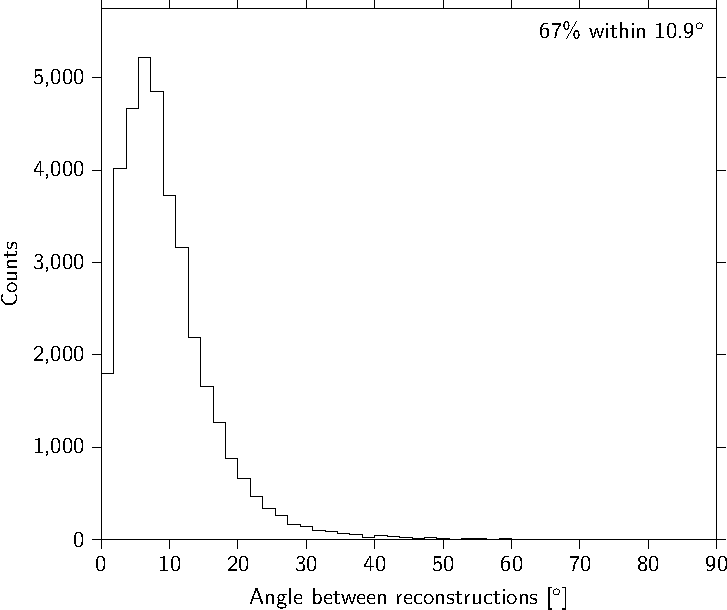
\includegraphics{plots/station/angle_between_501_510_minn2}
    \caption{Angle between the direction reconstruction in coincident events between station 501 and 510.}
    \label{fig:angle_between_501_510}
\end{figure}

